% =====================================================================
% LC-DeepONet — Draft v0.9 (SAGE sagej template, TIMC submission format)
%   Base content: main.tex (article class, Draft v0.8.2), unchanged except:
%   - Class switched to the official SAGE sagej.cls v1.20 (same directory;
%     file must accompany main_sagej.tex when compiling/submitting).
%   - Citations: Sage Vancouver numbered (superscript) per the CURRENT TIMC
%     guidelines; reference list reordered into first-citation order and
%     [author(year)] bibitem labels removed (Harvard formatting was based
%     on the outdated legacy instruction text).
%   - Headings unnumbered (SAGE house style); the 10 in-text
%     "Section~\ref{sec:...}" cross-references rewritten to named sections.
%   - Title block moved to sagej commands (\runninghead/\title/\author/
%     \affiliation/\corrauth/\email); abstract + \keywords placed before
%     \maketitle as the class requires. Keywords: "spectral normalization"
%     -> "spectral-norm penalty" (matches the corrected mechanism wording).
%   - Word budget unchanged (content edits are null-sum); limit 6000 words
%     / 10 illustrations per journals.sagepub.com/author-instructions/TIM.
% =====================================================================
% =====================================================================
% Lipschitz-Constrained DeepONet for Nonlinear System Identification
% and Small-Gain Robust Feedback Stabilization
%
% =====================================================================
% Draft v0.8 — 2026-09-18（按三位审稿人综合意见 review_v07_combined.md 修订）
%   (C-M1) 收回闭环"certified"表述：摘要 / Innovation 3 / Remark 3 / Remark 5 /
%          E6 / 结论统一为"模型增益 certified，被控对象与闭环层 calibrated"；
%          显式声明 safety factor 不把采样下界提升为上界，故不构成证书；
%   (C-M2) 明确 a posteriori 估计与 E6-A/B 扫描均在中值参数 (0.6,1.0,0.85) 评估；
%          新增 E6-C 参数箱 8 角点扫描（run_e6_corners.py）：eps_hat_L 变化 3.2x、
%          全部角点被覆盖、设计增益仅降 2%、9 个参数点闭环全稳定；新增 tab:e6c；
%   (C-M3) Theorem 1 增加采样保真前置条件（Remark 1 扩写 + Step 4 改写）：
%          证书对离散算子精确，连续 L2 结论需工作域带限（实验输入 16x 低于 Nyquist）；
%   (C-M4) 证据链统一：E2 区分 128 样本（tab:e1）与 512 样本（e2_ood.csv）两套 OOD；
%          tab:emap 增 M3/E6-C 行并去掉 "every" 绝对化；E4 DeepONet 1% std 0.0016→0.0024；
%          "FNO 最小 std" 改为 "仅次 MLP"；e4b_noise_5seed.csv 列错位 bug 修复并重生成；
%          run_all.py 扩展至 E1-E9 + M3；L_G_true 一律称 sampled lower-bound estimate；
%   (C-M5) 新增 Discussion "What the certificate buys, and what it costs" 段
%          （6.7x-7.7x 保守度、0.909-0.927 vs 0.255/2.97 跟踪误差、适用场景）；
%   (C-m1..m12) E4 std；E6 设计点 3.678/0.056 + e6_design_provenance.csv；
%          fig9 子标 (c)(d)；fig2 延迟符号 tau；fig3 面板(b) surrogate 标签；
%          RMSE 口径定义；notation table（tab:notation）；
%          E3 S_emp 全模型来源 + "可计算上界而非更小敏感度"的定位；
%          fig:accuracy 图注（相位滞后 + 小幅幅值偏差）；"delay-free"→one-step lag；
%          E5 措辞与 hinge 零激活自洽；Code availability 补齐映射与溯源说明；
%   (字数) 修订后初版 7107 词（正文 6808 + 摘要 299），超 TIMC 上限；经 _compress_pass1/2/3/4.py
%          四轮压缩（删除重复表述、收紧长句，不删任何数值/结论/引用/图表），终稿
%          正文 5527 + 摘要 294 = 5821 词；编译 25 页，0 error / 0 Overfull
%          / 0 undefined reference。官方页（2026-09-19 复核）原文为
%          "should not normally exceed 6000 words (with up to 10 illustrations)"，
%          并允许内容充分时超出，故 5821 处于可接受区间（如需压到 5000 需删实验分组，
%          与审稿意见要求的补内容方向相反，已在 SUBMISSION_CHECKLIST.md §5 给出削减顺序）。
% =====================================================================
% Draft v0.7 — 2026-09-17（投稿就绪版）
%   (m6) 图表合并 12→10（TIMC ≤10 图软规范）：fig4+fig5 合并为 fig:accuracy
%        (a)最差样本轨迹/(b)ID-OOD；fig8+fig9 合并为 fig:margin (a)-(d)
%        （(a)无延迟裕度扫描 (b)延迟扫描 (c)校准设计闭环轨迹 (d)未认证设计）；
%        tab:emap 与 E6-B 交叉引用同步更新；
%   - 字数审计：正文 5071 词 + 摘要 290 词 = 5361 ≤ 6000（TIMC 上限，达标）；
% Draft v0.6 — 2026-09-17（投稿目标：TIMC, SAGE, 中科院4区）
% 数值结果来自 LC-DeepONet/results/*.csv（E1-E9 正式实验；证书归属见 tab:emap）。
% v0.6 更新（据 review_report_simulated.md 模拟审稿，M1-M5 + m1-m8 逐条修复）：
%   (M1) E6(iii) S_emp 数值来源修正：0.254 实为 Transformer(seed43) 值，
%        改用 DeepONet 5-seed 均值 0.269±0.021（e3b_sensitivity_per_seed.csv），
%        k_c^opt 重算为 3.35（13.9× k_c^safe，原 3.54/14.7×）；
%   (M2) 新增 tab:routes 三路线对比表（model-free 1/Γ / a priori Cor.1 /
%        a posteriori 校准）+ Remark 4 互补性论证段（包络 ū≤0.176 vs 工作幅值）；
%   (M3) C_T 谱范数实测（run_m3_ctnorm.py，5 seeds）：L_cert 3.91±0.32(Fro)
%        → 3.31±0.29(spec)，降 15%；Theorem 1 Step 2 注记 + Discussion
%        Conservatism 段给出分解（branch 积 4.12 主导，C_T≈0.95）；
%   (M4) E7 lambda_lip 不敏感的结构性解释：探针实验证实 10 次训练 hinge
%        零激活（surrogate∈[1.5,3.8]<5），并澄清 E5 B-vs-A 差异来源
%        （幂迭代 RNG 流去相关 + seed 方差复现 0.0128±0.0023）；
%   (M5) Remark 3/5 显式声明 eps_hat_L 为 sampled lower bound 的后果 +
%        gamma_s∈{2,5,10} 数值（0.238/0.228/0.213，最多让步 12%）；
%   (m1) Theorem 2 补完整证明（修正显式界：分子含 (L_cert+eps_L)·L_C·||r||
%        因子，原稿遗漏）+ eq:sgbound；
%   (m2) Corollary 1 就地标注 double-counting（高度保守）；
%   (m3) fig:identification 图注/正文改为"误差性质检验"目的化表述；
%   (m4) tab:e5lam 注明 RMSE(4s) 基本平坦（max deviation 0.3%）；
%   (m5) E4 如实改为 LC 各噪声档略优（1% 档差距约 1 个 seed std）；
%   (m7) 新增 2 条 TIMC 自引（Liang et al. 2024, 46(6); Zheng 2024, 46(1)，
%        DOI 级核实）；
%   (m8) eps_hat_L 公式处就地标注 sampled lower bound；Prop 2 的 ||H|| 补
%        L2(R) induced-norm 说明；E6-B 0.909 消歧（指明为 E6-A(i) 无延迟值）。
%   m6（12 图合并至 ≤10）暂缓，留作返修选项。
% Draft v0.5 — 2026-09-17
% TIMC 格式适配（2026-09-17 定刊后）：
%   - Harvard 引用格式（natbib author-year，文献表字母序，18 条）；
%   - 摘要后新增 7 个关键词（TIMC 要求 ≥5）；\thanks 草稿残留清理；
%   - 单栏+图表嵌正文（TIMC 评审要求，现稿天然符合）。
% v0.5 更新（据 论文修改检查.pdf 投稿前硬伤修复，12 条意见）：
%   (1) 数字一致性：E1-E2 正文 OOD 数字统一为 Table 1（e1_identification.csv）；
%       "best mean RMSE among all baselines" 改为如实表述（MLP 0.0102 最优，
%       LC 与其相差 <1 个 seed 标准差）；
%   (2) L_cert 归属：新增 Experiment map 表（tab:emap）标注每处 L_cert 来源
%       （E1 demo 3.92 / E3 3.89±0.21 / E5-D 4.03±0.31 / E6 单run 3.68 /
%       E7 1.53-4.00 / E8 4.12±0.35, 3.37±0.08）；
%   (3) 理论：删除 Proposition 2(iii)（Grönwall 时间域论证不构成严格的
%       L2→L2 operator bound，采纳审稿方案A）；Theorem 1 补 trunk 维度
%       T(t)∈R^p；4.3 节明确 Lip ≤ L_cert 严格不等号（保守上界）；
%   (4) 措辞三层统一（Remark 3）：L_cert = certified upper bound on the
%       learned operator gain / eps_hat_L = empirical residual sensitivity
%       estimate / L_cert+eps_hat_L = empirically calibrated plant-gain
%       bound；Abstract 与 Conclusion 同步降调；
%   (5) E6：M<0 表述改为 loss of the theoretical guarantee（不宣称失稳，
%       与 Remark 5 一致）；新增 fig12 margin-RMSE 散点图（M=0 分界）；
%   (6) FNO 中性化（baseline 而非对手）；novelty 改 explicit-interface 表述；
%   (7) Abstract 补 3 个定量结果（L_cert≈3.9 / S_emp≈0.27 / 62% 压缩）；
%       E7 改名 Certificate-accuracy trade-off 且 Intro 提前提及；
%       E8 措辞改 without system-specific architecture changes；
%       RW 新增 learning-based ID & robust control 段 + gap table（tab:gap，
%       新增 7 条经核实的参考文献）。
% v0.4 更新（据 ChatGPT 终审第二轮，拟定SCI课题2.pdf）：
%   (1) Corollary 1 数学修正：eps_L := Gamma + L_hat（原 eps_L:=Gamma 推不出）；
%   (2) Remark 4 数值更新（0.086 vs 0.241，~2.8x）+ model-free 路线 1/Gamma；
%   (3) Remark 1 改写：eps_hat_L 定位为 empirical residual sensitivity estimate + gamma_s 安全系数；
%   (4) E6 重构：E6-A 无延迟（理论严格对应）+ E6-B 延迟 tau∈{50,100,200}ms；
%   (5) FNO 归因句软化；C1-C3 改名 Innovation 1-3；
%   (6) 术语清理：L_hat 全文定位为 certified upper bound（非 exact Lipschitz 常数）；
%   (7) E4 升级为 5 seeds（mean±std）；新增 E7：lambda_lip 不敏感 + L_target
%       Accuracy–Certificate trade-off（表 tab:e7 + fig10）；Limitations 相应收缩；
%       Setup 增加指向 E7 的说明。
% v0.4 更新（据 ChatGPT 终审第二轮，拟定SCI课题2.pdf）：
%   (1) L_hat 全文改名 L_cert（宏一处改定 + fig1/2/3/7/8 标签同步重生成）；
%   (2) E8 新增：Duffing + Pendulum 完整辨识 benchmark（3 模型 × 5 seeds，tab:e8）；
%   (3) E9 新增：long-horizon rollout（T=4/6s，RMSE(t) 曲线 fig11）；
%   (4) E5 升级 5 seeds + 新增 lambda_dyn 扫描（tab:e5lam）；叙事修正：
%       单罚项不涨精度、动态损失是稳定器（5-seed 结论与单 run 不同）；
%   (5) E3 升级 5 seeds（L_cert 3.89±0.21, S_emp 0.265±0.012, FNO 2.55±0.73）；
%   (6) Related Work novelty 三层对比强化（neural operators / Lipschitz NN /
%       neural-operator control）；E7 移至 E6 之后保持编号顺序；
%   (7) Limitations 再收缩（多系统与长时程已完成，余留 E6 单网络+delay 框架外）。
% v0.2 更新：
%   (1) Theorem 1 证明由 sketch 展开为完整证明；
%   (2) 新增 Proposition 2 + Corollary 1（假设 A1 对 MSD 类的先验论证）；
%   (3) Related Work 重写：区分 gain-kernel-approximation 与 operator-certificate 两条线；
%   (4) 参考文献逐条核实（Pauli/Bhan/Krstic/Xiao/Lv/Qi，含 DOI 级确认）。
% =====================================================================
\documentclass[11pt,sagev,times]{sagej}
% Options: 11pt -> article base size; sagev -> Sage Vancouver superscript
% numbered citations (natbib super,sort&compress); times -> Times/Helvetica.
% No paper-size option: Afour/MCfour/PCfour force \twocolumn, but TIMC
% guidelines require a single-column manuscript with all figures and tables
% within the text, so geometry is set explicitly below (A4, single column).
\usepackage[a4paper,margin=2.5cm]{geometry}
\usepackage{microtype}
\usepackage[hidelinks]{hyperref}
\hypersetup{
  pdftitle={Lipschitz-Constrained DeepONet for Nonlinear System Identification and Small-Gain Robust Feedback Stabilization},
  pdfauthor={Peng Chen},
  pdfsubject={Transactions of the Institute of Measurement and Control},
  pdfkeywords={nonlinear system identification; operator learning; DeepONet; Lipschitz constant; spectral-norm penalty; small-gain theorem; robust feedback control}
}
\usepackage{xurl}
\graphicspath{{../figures/}}

\newtheorem{theorem}{Theorem}
\newtheorem{proposition}{Proposition}
\newtheorem{corollary}{Corollary}
\newtheorem{assumption}{Assumption}
\newtheorem{remark}{Remark}
\newtheorem{lemma}{Lemma}

\newcommand{\Ltwo}{L^2}
\newcommand{\Ghat}{\hat{G}}
\newcommand{\Lhat}{L_{\mathrm{cert}}}
\newcommand{\epsL}{\varepsilon_L}
\newcommand{\LC}{L_{\mathrm{C}}}
\newcommand{\Ltarget}{L_{\mathrm{target}}}

% --- journal metadata (cosmetic; production resets these) ---
\def\volumeyear{2026}
\def\journalname{Trans.\ Inst.\ Meas.\ Control}

% --- SAGE sagej title block ---
\runninghead{LC-DeepONet: computable gain certificates for learning-based feedback design}
\title{Lipschitz-Constrained DeepONet for Nonlinear System Identification and Small-Gain Robust Feedback Stabilization}
\author{Peng Chen}
\affiliation{School of Computer Science, Xinyang University,
Xinyang 464000, Henan, China}
\corrauth{Peng Chen, School of Computer Science, Xinyang University,
Xinyang 464000, Henan, China. Email: 1192724829@qq.com.
ORCID iD: 0009-0004-9021-6039.}
\email{1192724829@qq.com}

\begin{document}

\begin{abstract}
Neural operators such as DeepONet learn mappings between infinite-dimensional
function spaces and have recently been applied to the identification of
nonlinear dynamic systems. However, a learned operator that fits trajectories well
provides \emph{no} computable certificate of its input--output gain, the
quantity required by robust-stability tools such as the small-gain theorem. We propose LC-DeepONet, a DeepONet whose
branch network carries a differentiable spectral-norm penalty on its gain and can be driven by a
$\sqrt{\Delta t}$-scaled input representation, so that an explicit, strictly
computable Lipschitz certificate $\Lhat$ for the learned operator in the
$\Ltwo$ operator-norm sense is obtained as a by-product of training. We then
make explicit a subtle distinction: a bound on the function-value error
$\|G-\Ghat\|_\infty$ does \emph{not} imply a bound on the Lipschitz constant
of the error operator; introducing the latter as an assumption yields a plant
gain bound $L_G\le \Lhat+\epsL$ --- a certified model gain plus a residual
term estimated from data, so the plant bound is \emph{empirically calibrated}
--- which feeds the small-gain condition $\LC(\Lhat+\epsL)<1$ for finite-gain
robust stability of the loop. On a parameter-uncertain nonlinear mass--spring--damper
system, the certified bound ($\Lhat\approx3.9$) encloses the measured
operator sensitivity ($\approx0.27$) with an order-of-magnitude margin at
matched identification accuracy without reducing that sensitivity, and its
training target tightens it by $62\%$ at essentially unchanged in-distribution
error. The same pipeline applies to Duffing and pendulum systems without
architecture changes. Closed-loop gain sweeps on the true plant show that the
predicted margin marks the boundary of the calibrated region and correlates
with the onset of the degraded response. The results form a chain --- operator
learning, model-gain certification, error bounding, gain-aware feedback
design --- in which the model gain alone is certified, while the plant- and
loop-level statements are empirically calibrated; on this plant the certificate
buys an offline gain-screening rule, not tracking performance.
\end{abstract}

\keywords{nonlinear system identification; operator learning; DeepONet; Lipschitz constant; spectral-norm penalty; small-gain theorem; robust feedback control}

\maketitle

% ---------------------------------------------------------------------




% ---------------------------------------------------------------------
\section{Introduction}\label{sec:intro}

Nonlinear systems are traditionally identified with parametric or
semi-parametric models whose stability properties classical tools can
analyze. Learning-based identifiers raise a new question: when the identifier
is a deep network, what does the identified model \emph{guarantee}? This paper
addresses the gap between \emph{what neural operators can fit} and \emph{what
feedback design can assume}.

Three deficiencies motivate this work.
\textbf{(i) Missing stability certificates.} Identification models are
evaluated by trajectory-fitting accuracy; the input--output gain that the
small-gain theorem requires is not provided.
\textbf{(ii) Uncontrolled sensitivity.} Sensitivity to input perturbations is
neither measured nor constrained during training, so an accurate model can
still amplify disturbances.
\textbf{(iii) Missing connection to closed-loop analysis.} How identification
error propagates into closed-loop robust stability remains largely
uncharacterized for general nonlinear systems beyond specific PDE settings.

% Gap statement (iii) verified against the neural-operator control
% literature of 2023--2025 (Bhan/Krstic, Qi/Krstic, Xiao, Lv); see Related
% Work for the precise positioning.

We address the three deficiencies with a single design: a
\emph{Lipschitz-constrained DeepONet} (LC-DeepONet) whose branch network is
trained under a differentiable spectral-norm penalty and whose input
representation is scaled by
$\sqrt{\Delta t}$, giving a directly computable $\Ltwo$ operator-gain
certificate $\Lhat$ (Proposed Method section). The certificate is converted
into a plant gain bound via an explicit Lipschitz bound on the error operator
(Stability Analysis section), and the bound feeds a small-gain condition for the
feedback loop (Fig.~\ref{fig:framework}). Beyond serving as a fixed
certificate, $\Lhat$ is itself \emph{designable}: a sweep over the constraint
target tightens the certificate by $62\%$ at essentially unchanged
identification error (E7), so the gain bound is an explicit design knob of
the training procedure rather than an emergent by-product.
At the default target of the identification and closed-loop baselines,
the hinge is inactive; the binding-target sweep in E7 is therefore the direct
evidence that the objective can actively tighten the certificate.

The contributions are:
\begin{enumerate}
  \item \textbf{Innovation 1 (Operator-level Lipschitz certificate).} An
  LC-DeepONet architecture that yields an
  explicit, strictly verifiable Lipschitz gain bound
  $\Lhat=(\prod_i \sigma(W_i))\, C_{\mathrm{T}}$ for the learned operator,
  where $\sigma(W_i)$ are spectral norms of the branch weights and
  $C_{\mathrm{T}}$ is the discrete $\Ltwo$ norm of the trunk basis.
  \item \textbf{Innovation 2 (Identification-error-to-gain interface).} A
  careful separation between the
  function-value error bound and the Lipschitz error bound of the residual
  operator $E=G-\Ghat$; under an explicit assumption on the latter, the
  certified plant bound $L_G\le\Lhat+\epsL$ follows.
  \item \textbf{Innovation 3 (Certificate-aware small-gain feedback).} A
  small-gain sufficient condition
  $\LC(\Lhat+\epsL)<1$ for finite-gain robust stability of the closed loop
  built on the learned model, together with a simulation protocol---a
  controller-gain sweep against the \emph{small-gain robustness margin}
  $M=1-\LC(\Lhat+\epsL)$---that empirically validates the margin's predictive
  value. The guarantee is hierarchical by construction: the model gain
  $\Lhat$ is certified, whereas the residual term $\epsL$ enters through
  Assumption~\ref{ass:residual} and, when estimated from data, makes the
  plant- and loop-level statements empirically calibrated rather than
  formally certified (Remarks~\ref{rem:epsL} and~\ref{rem:claim}).
\end{enumerate}

The paper is deliberately positioned as a simulation-based methodological
study; hardware validation is left as future work.

% ---------------------------------------------------------------------
\section{Related Work}\label{sec:related}

\textbf{Neural operators.} DeepONet~\citep{lu2021deeponet} approximates
operator mappings via a branch--trunk architecture; the Fourier Neural
Operator~\citep{li2021fno} learns in spectral space. Both serve here as
baselines and as the method backbone. This line targets approximation
accuracy and resolution transfer, with theory now well developed
\citep{lanthaler2022error}; the
trained operator carries no computable gain information that a feedback design
could consume. Certification for DeepONets has so far been pursued as
uncertainty quantification \citep{moya2025conformal}, not as a deterministic
input--output gain bound.

\textbf{Neural operators in feedback control.} A growing line uses neural
operators to \emph{approximate gain kernels} inside PDE backstepping
syntheses, introduced by Bhan et al.\ for plant-coefficient mappings and
extended to controller and observer gains for reaction--diffusion PDEs
\citep{bhan2024bypassing,krstic2024observer}, with further applications to hyperbolic
output regulation, cascaded parabolic PDEs, and a hyperbolic PIDE with recycle
and delay \citep{xiao2024output,lv2025cascaded,qi2024pide}.
The network there is a function approximator \emph{inside} a proof tied to a
specific PDE class, carrying no reusable computable gain. Our work differs in
three respects: the plant class is general finite-dimensional rather than
PDE-specific; the certificate is a property of the learned operator itself
rather than of an approximated kernel; and the stability argument is the
classical small-gain theorem, consumable by any controller with a known gain.

\textbf{Lipschitz-constrained networks.} Spectral
normalization~\citep{miyato2018spectral} and 1-Lipschitz activation
architectures~\citep{pauli2021lipschitz} bound the Lipschitz constant of
finite-dimensional maps, for robust certification and robust MPC. Those
certificates concern Euclidean maps; lifting them to function spaces requires
the discretization-consistent scaling introduced in the Proposed Method section and yields a
gain that the small-gain theorem, rather than a robust-control synthesis,
consumes directly. The contribution here is the \emph{explicit interface} between the two lines:
an operator-level certificate attached to a trained DeepONet and converted,
through an identification-error-to-plant-gain bound, into a small-gain
condition.

\textbf{Learning-based system identification and robust control.} A broad
line of work builds data-driven models and controllers with stability in
mind: sparse and physics-informed identification
\citep{brunton2016sindy,raissi2019pinn}, learned state-space models
\citep{lusch2018deep,masti2021learning}, stable deep dynamics and neural
Lyapunov functions \citep{kolter2019learning,chang2019neural}, adaptive
neural control \citep{liang2024learning,zheng2024adaptive}, and
learning-based MPC with safety guarantees \citep{hewing2020learning}. These
deliver accurate models, stable dynamics, or state-space certificates; none
provides a computable input--output \emph{gain} certificate for a
generic learned operator that a small-gain design can consume
(Table~\ref{tab:gap}).

\begin{table}[t]
\centering\small
\caption{Positioning relative to adjacent lines of work.}
\label{tab:gap}
\begin{tabular}{p{4.6cm}p{2.4cm}p{2.6cm}p{2.4cm}}
\toprule
Line of work & Operator-level ($\Ltwo$ I/O) & Computable gain bound & General plant class \\
\midrule
Neural operators \citep{lu2021deeponet,li2021fno} & \checkmark & -- & \checkmark \\
Neural-operator PDE control \citep{bhan2024bypassing,krstic2024observer} & \checkmark & kernel-specific & PDE class \\
Lipschitz-constrained networks \citep{miyato2018spectral,pauli2021lipschitz} & -- & \checkmark & finite-dim.\ maps \\
Neural Lyapunov / stable dynamics \citep{chang2019neural,kolter2019learning} & -- & -- & state space \\
\textbf{This work} & \checkmark & \checkmark & \checkmark \\
\bottomrule
\end{tabular}
\end{table}

\textbf{Small-gain theorem.} The classical input--output stability framework
\citep{desoer1975feedback,khalil2002nonlinear} provides the tool by which our
certified gain becomes a stability guarantee. We do not modify the theorem;
the contribution is making its hypothesis computable for learned operators.
Table~\ref{tab:notation} collects the symbols used throughout the paper.

% ---------------------------------------------------------------------
\section{Preliminaries}\label{sec:prelim}

\subsection{System and operator formulation}
Consider the nonlinear system
\begin{equation}
  \dot{x}(t) = f(x(t),u(t),\mu),\qquad y(t) = h(x(t)),\qquad t\in[0,T],
\end{equation}
with uncertain parameter $\mu$, and its input--output operator
$G:\mathcal{U}\to\mathcal{Y}$ with
$\mathcal{U}=\Ltwo([0,T])$, $\mathcal{Y}=\Ltwo([0,T])$. The identification
goal is a learned operator $\Ghat_\theta\approx G$ from input--output data.

\subsection{Lipschitz operators}
$G$ is Lipschitz on $\mathcal{D}\subseteq\mathcal{U}$ if
$\|G(u_1)-G(u_2)\|_{\mathcal{Y}}\le L_G\|u_1-u_2\|_{\mathcal{U}}$ for all
$u_1,u_2\in\mathcal{D}$; the infimum of such $L_G$ is $\mathrm{Lip}(G)$.
For a composition of maps, constants multiply.

\subsection{Small-gain theorem}
For a feedback interconnection $e_1=u_1-S_2(e_2)$, $e_2=u_2+S_1(e_1)$ with
causal, finite-gain, well-posed $S_1,S_2$, if $\mathrm{Lip}(S_1)\,
\mathrm{Lip}(S_2)<1$ then the closed loop is finite-gain stable with explicit
gain bounds \citep{desoer1975feedback,khalil2002nonlinear}.

\begin{table}[t]
\centering\small
\caption{Notation. Every symbol is also defined at its first use; this table
is provided for reference.}
\label{tab:notation}
\begin{tabular}{ll}
\toprule
Symbol & Meaning \\
\midrule
$G$, $\Ghat$ & true plant operator and learned operator $\Ghat_\theta$ \\
$E=G-\Ghat$ & residual (plant--model mismatch) operator \\
$\mathrm{Lip}(\cdot)$ & induced Lipschitz gain (the $\Ltwo$ operator norm) \\
$\Lhat$ & certified upper bound on $\mathrm{Lip}(\Ghat)$, equal to
$\big(\prod_i\sigma(W_i)\big)C_{\mathrm{T}}$ \\
$\sigma(W_i)$ & exact spectral norm of branch layer $i$ (SVD at evaluation time) \\
$C_{\mathrm{T}}$ & trunk constant $\big(\Delta t\sum_j\|T(t_j)\|_2^2\big)^{1/2}$ (Frobenius form) \\
$\epsL$, $\hat\epsL$ & residual Lipschitz constant of Assumption~\ref{ass:residual},
and its sampled lower-bound estimate \\
$\widehat{\mathrm{Lip}}(G)$ & sampled lower-bound estimate of the true plant
gain $\mathrm{Lip}(G)$, reported as $L_G$ \\
$\gamma_s$ & heuristic safety factor on $\hat\epsL$,
$\gamma_s\in\{2,5,10\}$ \\
$\Gamma$ & a priori plant-gain bound of Proposition~\ref{prop:apriori} \\
$S_{\mathrm{emp}}$ & empirical input-perturbation sensitivity of a trained model \\
$\LC$ & Lipschitz gain of the controller $C$ \\
$k_c$ & static output-feedback gain, $u=k_c(r-y)$ \\
$M$ & small-gain robustness margin, $1-k_c(\Lhat+\hat\epsL)$ \\
$\Ltarget$ & training target for the surrogate certificate in \eqref{eq:loss} \\
$N$, $\Delta t$ & samples per window and sampling interval, $\Delta t=T/N$ \\
\bottomrule
\end{tabular}
\end{table}

% ---------------------------------------------------------------------
\section{Proposed Method: LC-DeepONet}\label{sec:method}

\subsection{DeepONet formulation}
The DeepONet output at query time $t_j$ is
\begin{equation}
  \Ghat(u)(t_j) \;=\; \sum_{k=1}^{p} B_k(u)\, T_k(t_j) + b_j,
  \label{eq:deeponet}
\end{equation}
where $B(u)=[B_1(u),\dots,B_p(u)]^\top$ is produced by the \emph{branch}
network from the discretized input $u=[u(t_0),\dots,u(t_{N-1})]^\top$ and
$T(t)=[T_1(t),\dots,T_p(t)]^\top$ by the \emph{trunk} network from the query
time.

\subsection{$\sqrt{\Delta t}$-consistent input scaling}
\begin{remark}[Discrete-$\Ltwo$ consistency and the working domain]\label{rem:sqrtdt}
With uniform sampling $t_j=j\Delta t$,
$\|u\|_{\Ltwo([0,T])}\approx\sqrt{\Delta t}\,\|u\|_{\ell^2}$.
The branch network therefore receives the scaled input
$z=\sqrt{\Delta t}\,u$, so that its Euclidean Lipschitz constant
$\mathrm{Lip}(B)$ acts directly as the operator-space constant:
$\|B(u_1)-B(u_2)\|_2\le\mathrm{Lip}(B)\,\|u_1-u_2\|_{\Ltwo}$.
Omitting this scaling decouples the certificate from the physical norm and
invalidates the bound of Theorem~\ref{thm:cert}.

The branch network also sees only the $N$ samples $u(t_j)$, so the bound of
Theorem~\ref{thm:cert} is \emph{exact for the discrete operator} mapping a
sample vector to a sample vector. Its transfer to the continuous operator
$\Ltwo([0,T])\to\Ltwo([0,T])$ needs a sampling-fidelity condition on the
working domain: $\mathcal{D}$ must consist of signals faithfully represented by
their samples, e.g.\ signals band-limited below the Nyquist rate
$1/(2\Delta t)$ (the experimental inputs are three tones in $[0.2,2]$\,Hz
against a $32$\,Hz sampling rate, i.e.\ $16\times$ below Nyquist), or signals
defined on the fixed grid. Under that condition the two norms agree on
$\mathcal{D}$; without it $\Lhat$ bounds the discrete operator only and the
continuous statement holds in the $\Delta t\to0$ limit. The condition matters
because two continuous inputs that coincide at the sample points but differ in
between have zero discrete distance and non-zero $\Ltwo$ distance, and the
certificate cannot control a difference it cannot see.
\end{remark}

\subsection{Spectrally constrained branch and certificate}
Each linear layer $W_i$ of the branch is trained with a differentiable
spectral penalty; at evaluation time the exact spectral norm
$\sigma(W_i)=\|W_i\|_2$ is used. With $1$-Lipschitz activations (ReLU),
$\mathrm{Lip}(B)\le\prod_i \sigma(W_i)$. The training objective is
\begin{equation}
  \mathcal{L} = \mathcal{L}_{\mathrm{data}}
  + \lambda_{\mathrm{dyn}}\mathcal{L}_{\mathrm{dyn}}
  + \lambda_{\mathrm{lip}}\max\!\big(0,\,\Lhat-\Ltarget\big)^2,
  \label{eq:loss}
\end{equation}
where $\mathcal{L}_{\mathrm{dyn}}$ enforces consistency of the network-output
derivative with measured $\dot q$, and $\Lhat$ is the \emph{differentiable}
surrogate bound (power iteration) --- the certified bound is evaluated
only for evaluation and for the closed-loop design. This separation is
essential: a no-grad bound inside the loss would receive no gradient. It also
fixes the status of the penalty: at the default target ($\Ltarget=5$) the
surrogate never reaches it, so the hinge is inactive in every run reported
here; the penalty is a safeguard that becomes the effective constraint only
when the target is tightened (E7).

Throughout, $\Lhat$ is a \emph{certified upper bound} on
$\mathrm{Lip}(\Ghat)$: the guarantee is $\mathrm{Lip}(\Ghat)\le\Lhat$ ---
equality is neither claimed nor used anywhere --- it is provably valid
(Theorem~\ref{thm:cert}) and is evaluated exactly from the weights via SVD,
but it is in general not the \emph{minimal} Lipschitz constant of $\Ghat$;
the resulting conservatism is quantified in the Numerical Experiments section.

\subsection{Operator-level certificate}
\begin{theorem}[Lipschitz certificate]\label{thm:cert}
Let the branch layers satisfy $\sigma(W_i)\le s_i$ and let activations be
$1$-Lipschitz. Define
$C_{\mathrm{T}}=\big(\Delta t\sum_{j}\|T(t_j)\|_2^2\big)^{1/2}$, where
$T(t_j)\in\mathbb{R}^p$ are the trunk features of \eqref{eq:deeponet} at
the sample points $t_j$.
Then for all $u_1,u_2$ in the working domain $\mathcal{D}$, provided
$\mathcal{D}$ satisfies the sampling-fidelity condition of
Remark~\ref{rem:sqrtdt},
\begin{equation}
  \|\Ghat(u_1)-\Ghat(u_2)\|_{\Ltwo([0,T])}
  \;\le\; \underbrace{\Big(\prod_i s_i\Big) C_{\mathrm{T}}}_{=\;\Lhat}\;
  \|u_1-u_2\|_{\Ltwo([0,T])}.
\end{equation}
\end{theorem}
\begin{proof}
Write $\delta u = u_1-u_2$, $\delta B = B(u_1)-B(u_2)$, and
$\delta\Ghat(t_j) = \Ghat(u_1)(t_j)-\Ghat(u_2)(t_j)$.

\emph{Step 1 (pointwise bound in the coefficient space).} By
\eqref{eq:deeponet}, the offset $b_j$ is input-independent and cancels, so
$\delta\Ghat(t_j) = \delta B^{\top} T(t_j)$. The Cauchy--Schwarz
inequality in $\mathbb{R}^p$ gives, for every $j$,
\begin{equation}
  |\delta\Ghat(t_j)| \;\le\; \|\delta B\|_2\,\|T(t_j)\|_2 .
  \label{eq:pointwise}
\end{equation}

\emph{Step 2 (trunk aggregation).} Squaring \eqref{eq:pointwise}, summing
over $j$ with weight $\Delta t$, and taking square roots,
\begin{equation}
  \|\delta\Ghat\|_{\ell^2_{\Delta t}}
  \;\le\; \|\delta B\|_2\,
  \Big(\Delta t\sum_j \|T(t_j)\|_2^2\Big)^{\!1/2}
  \;=\; \|\delta B\|_2\, C_{\mathrm{T}} .
  \label{eq:trunkbound}
\end{equation}
Note that $C_{\mathrm{T}}$ is the $\Delta t$-weighted Frobenius norm of the
trunk matrix, which upper-bounds its spectral norm: the certificate is
therefore conservative but computable from weights alone. Replacing it by
$\|\Phi_T\|_2=\sqrt{\lambda_{\max}(\Phi_T^{\top}\Phi_T)}$, where
$\Phi_T$ stacks the rows $\sqrt{\Delta t}\,T(t_j)^{\top}$, gives a
strictly tighter bound of the same form (the aggregation step is unchanged):
on the default MSD configuration it lowers the certificate from
$\Lhat=3.91\pm0.32$ (Frobenius) to $3.31\pm0.29$ over five seeds (sample
standard deviations; \texttt{results/m3\_ctnorm\_per\_seed.csv}), a $15\%$
reduction (Discussion section). We retain the Frobenius form
because it admits the closed-form $\Delta t$-weighted expression and the
differentiable surrogate used in training, and all reported certificates use
it consistently.

\emph{Step 3 (branch bound).} The branch computes
$B(u) = W_L\,\phi\!\big(W_{L-1}\cdots\phi(W_1 z)\cdots\big)$ with
$z=\sqrt{\Delta t}\,u$ (Remark~\ref{rem:sqrtdt}) and $1$-Lipschitz
activation $\phi$, applied componentwise. For any two intermediate
activations $a,b$,
\begin{equation}
  \|W_i\phi(a)-W_i\phi(b)\|_2
  \;\le\; \sigma(W_i)\,\|\phi(a)-\phi(b)\|_2
  \;\le\; \sigma(W_i)\,\|a-b\|_2 ,
\end{equation}
since $\phi$ is $1$-Lipschitz componentwise. Applying this inequality
recursively from the input layer to the output layer (a telescoping
product),
\begin{equation}
  \|\delta B\|_2 \;\le\; \Big(\prod_{i=1}^{L}\sigma(W_i)\Big)\|z_1-z_2\|_2
  \;=\; \Big(\prod_{i=1}^{L}\sigma(W_i)\Big)\sqrt{\Delta t}\,\|\delta u\|_{\ell^2}
  \;\le\; \Big(\prod_{i=1}^{L} s_i\Big)\,\|\delta u\|_{\ell^2_{\Delta t}} .
  \label{eq:branchbound}
\end{equation}

\emph{Step 4 (discrete-to-continuous).} Substituting
\eqref{eq:branchbound} into \eqref{eq:trunkbound} gives
\[
\|\Ghat(u_1)-\Ghat(u_2)\|_{\ell^2_{\Delta t}}
\;\le\; \Big(\prod_i s_i\Big)\,C_{\mathrm{T}}\,\|\delta u\|_{\ell^2_{\Delta t}}.
\]
Both the input and the output norms are evaluated in the same discretized
$\Ltwo$ sense, and
$\|\cdot\|_{\ell^2_{\Delta t}}\to\|\cdot\|_{\Ltwo([0,T])}$ as
$\Delta t\to0$ (Remark~\ref{rem:sqrtdt}). Hence $\Lhat=(\prod_i s_i)\,
C_{\mathrm{T}}$ is a rigorous upper bound for the discrete operator, and it is
a bound for the continuous $\Ltwo([0,T])$ operator on any working domain
$\mathcal{D}$ that satisfies the sampling-fidelity condition of
Remark~\ref{rem:sqrtdt}; on general $\Ltwo([0,T])$ inputs the continuous
statement is the corresponding $\Delta t\to0$ limit.
\end{proof}

\begin{figure}[t]
\centering
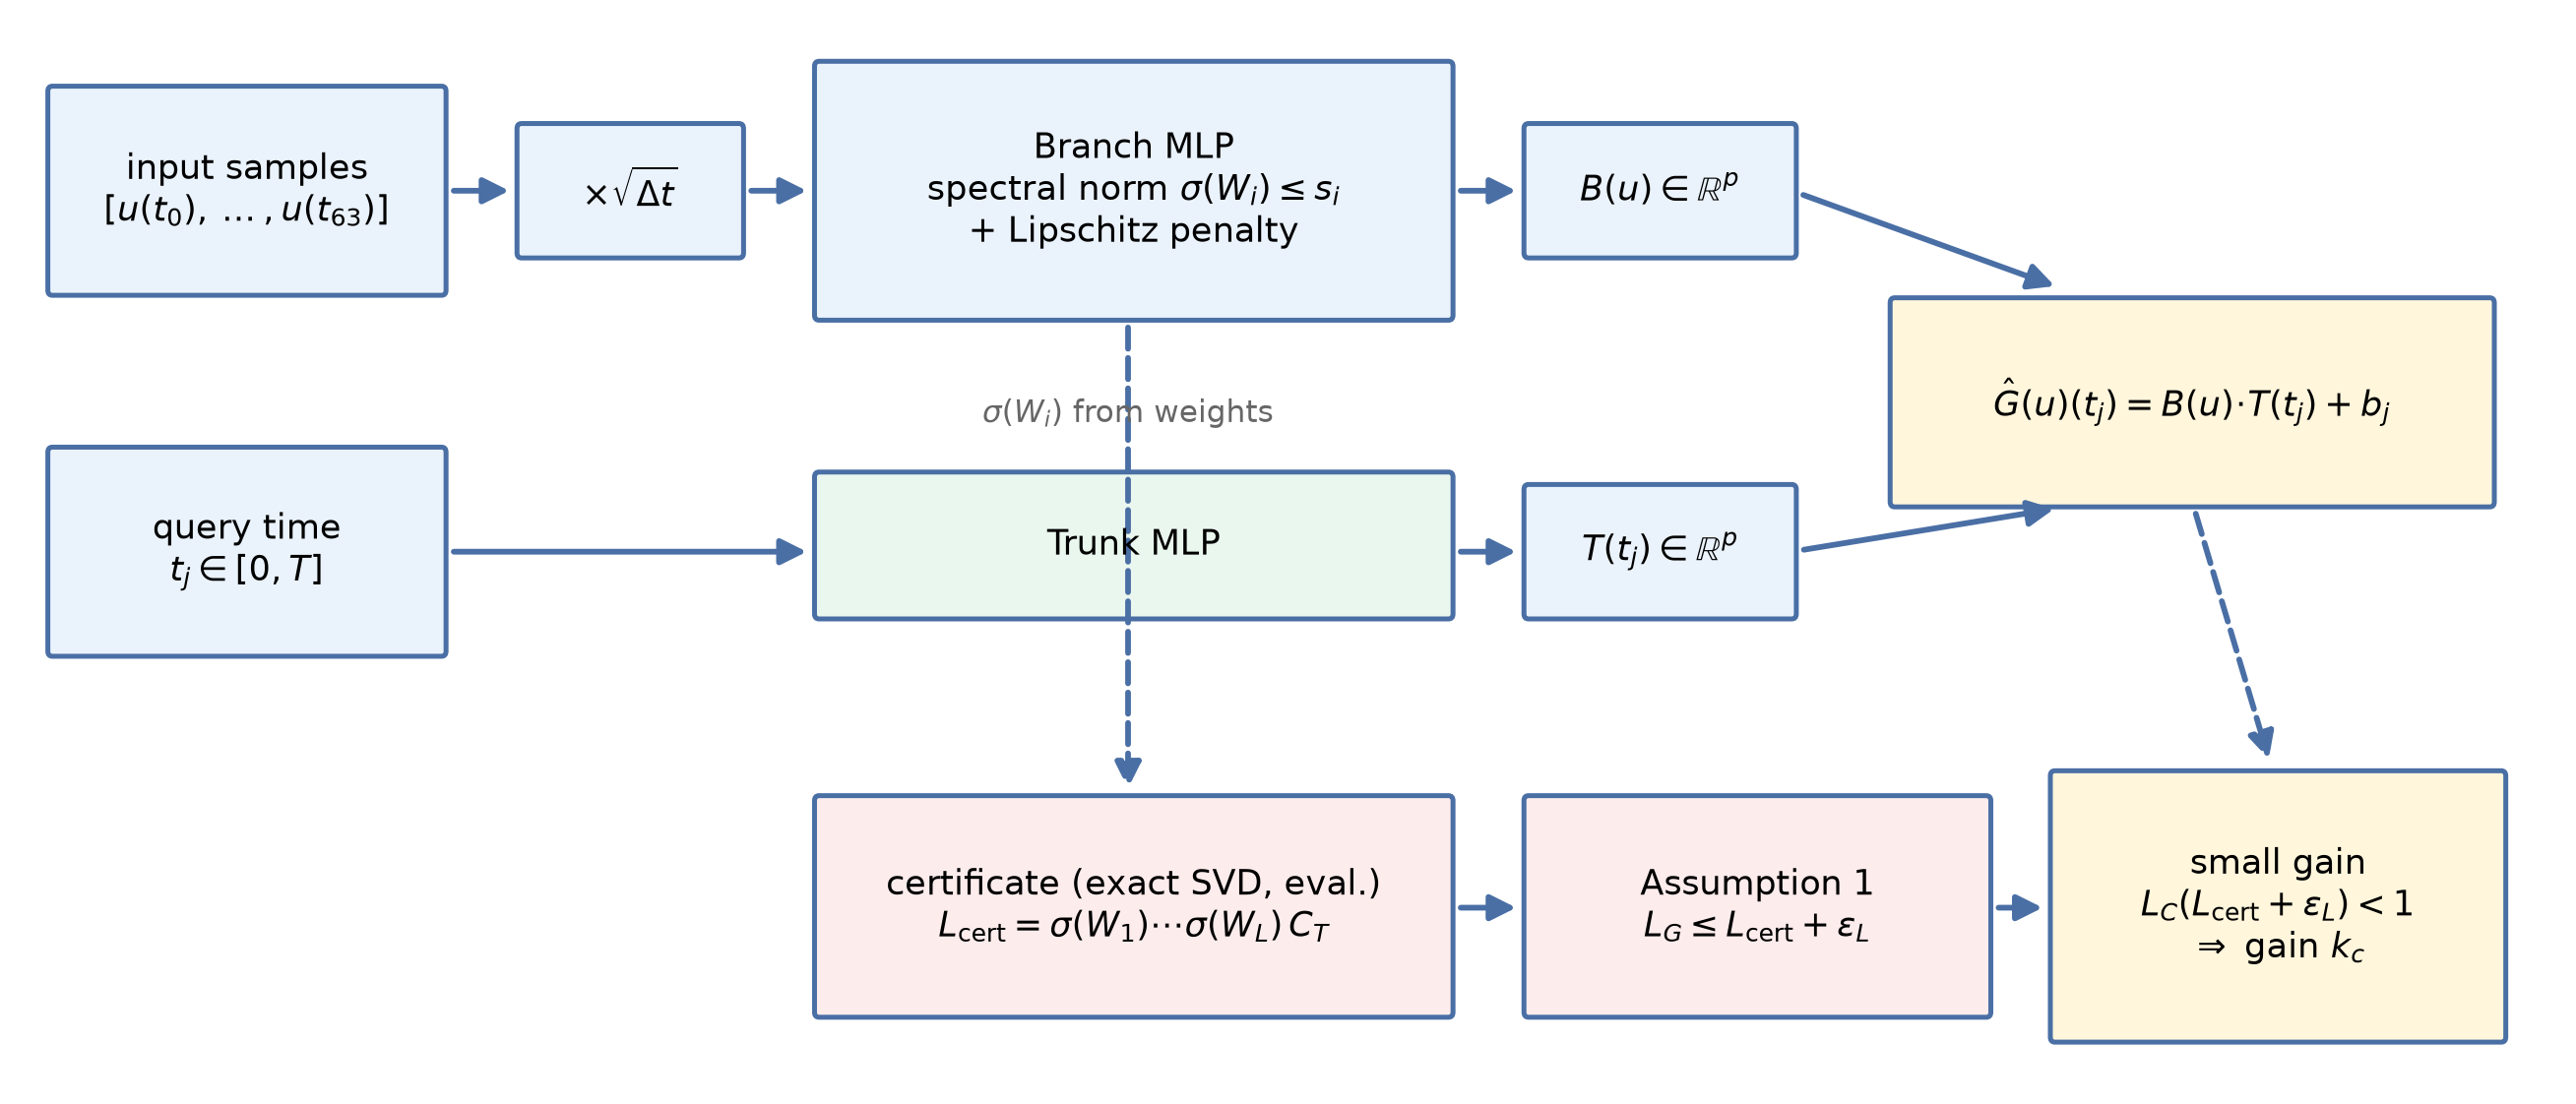
\includegraphics[width=\textwidth]{fig1_framework.png}
\caption{Overview of the proposed framework. Top: the LC-DeepONet
identifier---the branch network receives the $\sqrt{\Delta t}$-scaled input
and is spectrally constrained, so the weight-based certificate
$\Lhat=(\prod_i\sigma(W_i))\,C_{\mathrm{T}}$ (bound evaluated exactly via
SVD at evaluation time)
is a by-product of training. Bottom: the certificate chain---the residual
assumption (Assumption~\ref{ass:residual}) converts $\Lhat$ into a plant
gain bound, and the small-gain condition sizes the admissible loop gain.}
\label{fig:framework}
\end{figure}

% ---------------------------------------------------------------------
\section{Robust Identification and Stability Analysis}\label{sec:theory}

\subsection{Value error vs.\ Lipschitz error}
\begin{remark}[A common but invalid shortcut]\label{rem:invalid}
A uniform value-error bound $\sup_u\|G(u)-\Ghat(u)\|\le\varepsilon$ does
\emph{not} imply $\mathrm{Lip}(G-\Ghat)\le\varepsilon$, nor does it imply
$\mathrm{Lip}(G)\le\mathrm{Lip}(\Ghat)+\varepsilon$. The two bounds live in
different spaces: one bounds function values, the other bounds the induced
gain of the residual operator. Conflating them produces certificates that
cannot be defended in review.
\end{remark}

\begin{assumption}[Lipschitz residual]\label{ass:residual}
There exists $\epsL<\infty$ such that the residual operator
$E=G-\Ghat$ satisfies
$\|E(u_1)-E(u_2)\|_{\mathcal{Y}}\le\epsL\|u_1-u_2\|_{\mathcal{U}}$
for all $u_1,u_2$ in the working domain $\mathcal{D}$.
\end{assumption}

\begin{proposition}[Certified plant gain]\label{prop:gain}
Under Theorem~\ref{thm:cert} and Assumption~\ref{ass:residual},
\begin{equation}
  \mathrm{Lip}(G)\;\le\;\Lhat+\epsL .
\end{equation}
\end{proposition}
\begin{proof}
$\|G(u_1)-G(u_2)\|
\le\|\Ghat(u_1)-\Ghat(u_2)\|+\|E(u_1)-E(u_2)\|
\le(\Lhat+\epsL)\|u_1-u_2\|$.
\end{proof}

\begin{remark}[Estimating $\epsL$]\label{rem:epsL}
$\epsL$ is estimated empirically as
$\hat\epsL=\max_{i\ne j}\|E(u_i)-E(u_j)\|_{\Ltwo}/\|u_i-u_j\|_{\Ltwo}$ over a
domain-covering input pool; as a maximum over a finite sample it is a
\emph{sampled lower bound} on the true Lipschitz constant of $E$ over
$\mathcal{D}$, so $\hat\epsL$ is an \emph{empirical residual sensitivity
estimate}, not a certificate, and designs based on it are \emph{empirically
calibrated} rather than formally certified. A heuristic safety factor
$\epsL^{\mathrm{safe}}:=\gamma_s\hat\epsL$ with, e.g.,
$\gamma_s\in\{2,5,10\}$ reduces the admissible gain and biases the design
towards caution, but does \emph{not} convert the sampled lower bound into an
upper bound: nothing guarantees $\gamma_s\hat\epsL\ge\mathrm{Lip}(E)$, so
the inflated quantity is a heuristic hedge and the design rule remains
\emph{sample-calibrated} (its price is quantified in
Remark~\ref{rem:claim}).
The terminology used throughout this paper is fixed accordingly:
$\Lhat$ is a \emph{certified upper bound on the learned operator gain};
$\hat\epsL$ is an \emph{empirical residual sensitivity estimate}; and their
sum $\Lhat+\hat\epsL$ is an \emph{empirically calibrated plant-gain
bound}, not a formal certificate of the closed loop.
\end{remark}

\subsection{A priori bound on $\epsL$ for the MSD plant class}
\label{sec:apriori}
Assumption~\ref{ass:residual} constrains \emph{nature}, and so far it can
only be checked a posteriori from data (Remark~\ref{rem:epsL}). For
structured plant classes it can additionally be made explicit \emph{a
priori}, from the parameter ranges alone; for the mass--spring--damper class
used here the argument combines an energy estimate, a sector bound on the
nonlinearity, and a Neumann-series contraction through the nominal linear
operator.

\begin{proposition}[A priori gain bound for the MSD class]\label{prop:apriori}
Let $P$ be the plant $q''+c\,q'+k\,q+\alpha q^3=u$ with zero initial
conditions, parameters in the box
$[c_{\min},c_{\max}]\times[k_{\min},k_{\max}]\times(0,\alpha_{\max}]$, and
inputs in the class
$\mathcal{U}_{\bar u}=\{u\in\Ltwo([0,T]):\|u\|_\infty\le\bar u\}$ on the
finite horizon $[0,T]$. Then:
(i) every trajectory satisfies the pointwise state bound
\begin{equation}
  |q(t)| \;\le\; \bar M \;=\; \bar u\,\sqrt{\frac{T}{2\,k_{\min}c_{\min}}};
  \label{eq:Mbar}
\end{equation}
(ii) if
$\rho:=3\alpha_{\max}\bar M^2\,\|H\|_{\Ltwo\to\Ltwo}<1$, where $H$ denotes
the linear mass--spring--damper operator $\ddot q+c\dot q+kq=w$ with the
same $(c,k)$ and
$\|H\|_{\Ltwo\to\Ltwo}=\sup_\omega\big|(k-\omega^2+jc\omega)^{-1}\big|$
(the induced norm of the linear MSD on $L^2(\mathbb{R})$; finite-horizon
signals are extended by zero in the proof, so this serves as a uniform
bound for the truncated operator),
then
\begin{equation}
  \mathrm{Lip}(P)\;\le\;\Gamma \;:=\;
  \frac{\|H\|_{\Ltwo\to\Ltwo}}{1-\rho};
  \label{eq:Gamma}
\end{equation}
i.e., under the contraction condition $\rho<1$ the plant operator is
Lipschitz on the prescribed operating envelope, with the explicit constant
$\Gamma$.
\end{proposition}

\begin{proof}
\emph{(i) Energy estimate.} With unit mass and the energy
$V=\tfrac12\dot q^2+\tfrac12kq^2+\tfrac14\alpha q^4$,
\begin{equation}
  \dot V = \dot q\,(u-c\dot q) \;\le\; \bar u\,|\dot q| - c\,\dot q^2
  \;\le\; \frac{\bar u^2}{4c},
\end{equation}
where the last step maximizes the concave quadratic in $|\dot q|$. Since
$\tfrac12 kq^2\le V$ and $V(0)=0$ (zero initial conditions),
$|q(t)|^2\le 2V(t)/k \le \bar u^2T/(2ck)$; the right-hand side is largest
at $c_{\min},k_{\min}$, giving \eqref{eq:Mbar}.

\emph{(ii) Sector bound and contraction.} With zero initial conditions,
both trajectories satisfy the convolution representation
$q_i=H(u_i-\alpha q_i^3)$, $i=1,2$; subtracting,
\begin{equation}
  \delta q \;=\; H\big(\delta u-\alpha(q_1^3-q_2^3)\big),
  \qquad \delta q = q_1-q_2,\;\; \delta u = u_1-u_2 .
\end{equation}
On $\mathcal{U}_{\bar u}$, both $|q_i|\le\bar M$ by (i), so the pointwise
sector bound
$|q_1^3-q_2^3|=|q_1-q_2|\,|q_1^2+q_1q_2+q_2^2|\le 3\bar M^2\,|\delta q|$
holds. Applying $H$, using the triangle inequality and the induced-norm
bound (the signals are extended by zero to $\mathbb{R}$, for which the
$\Ltwo(\mathbb{R})\to\Ltwo(\mathbb{R})$ norm of the linear MSD equals
$\sup_\omega|(k-\omega^2+jc\omega)^{-1}|$),
\begin{equation}
  \|\delta q\|_{\Ltwo}
  \;\le\; \|H\|_{\Ltwo\to\Ltwo}\big(\|\delta u\|_{\Ltwo}
  + 3\alpha_{\max}\bar M^2\,\|\delta q\|_{\Ltwo}\big),
\end{equation}
which rearranges to \eqref{eq:Gamma} whenever $\rho<1$.
\end{proof}

\begin{corollary}[A priori $\epsL$]\label{cor:apriori}
Under Proposition~\ref{prop:apriori}(ii), the residual operator
$E=G-\Ghat$ of Assumption~\ref{ass:residual} satisfies, by the triangle
inequality,
$\mathrm{Lip}(E)\le\mathrm{Lip}(P)+\mathrm{Lip}(\Ghat)\le\Gamma+\Lhat$.
Hence Assumption~\ref{ass:residual} holds \emph{a priori} with the
plant-data-free choice
\begin{equation}
  \epsL \;:=\; \Gamma + \Lhat ,
  \label{eq:epsL-apriori}
\end{equation}
a bound that is \emph{highly conservative} because it double-counts the
certificate: $G$ and $\Ghat$ are strongly correlated ($\Ghat$ approximates
$G$), yet the triangle inequality adds their Lipschitz constants as if
they were independent (cf.\ Remark~\ref{rem:price}).
Theorem~\ref{thm:sg} then admits any controller with
$\LC<1/(2\Lhat+\Gamma)$. Alternatively, one may bypass the learned model
entirely within the envelope and combine
Proposition~\ref{prop:apriori}(ii) directly with the small-gain condition,
which admits $\LC<1/\Gamma$; the learned certificate is not needed on this
path.
\end{corollary}

\begin{remark}[The price of a priori certification]\label{rem:price}
For the experimental MSD box ($c\in[0.4,0.8]$, $k\in[0.8,1.2]$,
$\alpha\le1.2$, $T=2$\,s) the constants evaluate to
$\|H\|_{\Ltwo\to\Ltwo}\le 1/(c_{\min}\sqrt{k_{\min}-c_{\min}^2/4})=2.87$
(the resonant peak; $k>c^2/2$ throughout the box, so every member possesses
one), $\bar M=1.77\,\bar u$, and $\rho=32.3\,\bar u^2$, so the a priori
envelope is $\bar u<0.176$. At $\bar u=0.1$, $\Gamma=4.23$ and the a priori
choice \eqref{eq:epsL-apriori} gives $\epsL=\Gamma+\Lhat=7.91$, hence an
admissible loop gain $\LC<1/(2\cdot3.68+4.23)\approx0.086$ versus $0.241$
from the a posteriori calibration in the Numerical Experiments section --- a
factor of $\approx2.8$ paid for not using data. The model-free route
$\LC<1/\Gamma\approx0.24$ is comparable but confined to the same
small-signal envelope. The experimental inputs (three superposed sinusoids,
$\|u\|_\infty$ up to $3$, some $17\times$ that envelope) lie far outside
it: the state-dependent stiffness $\alpha\,(q_1^2+q_1q_2+q_2^2)$ makes the
error dynamics a \emph{time-varying} system for which no simple
frequency-domain bound holds globally. The framework therefore pairs the two
routes: the a priori envelope needs no data but covers only small signals
(and, by the triangle inequality, double-counts the certificate), whereas
the a posteriori estimator covers the operating amplitude but is a lower
bound and consumes a safety factor. Table~\ref{tab:routes} juxtaposes them.
The near-coincidence of $1/\Gamma\approx0.24$ and the calibrated $0.241$ is
incidental to this box and carries no structural meaning. Within the
envelope, a practitioner who does not need a learned model should prefer the
model-free route; the certificate route exists for the amplitude regime
where no envelope bound is available, and it returns the trained operator
alongside the bound.
\end{remark}

\begin{table}[t]
\centering\small
\caption{Three routes to a plant-gain bound for the MSD box of
Remark~\ref{rem:price} ($\Gamma=4.23$, $\Lhat=3.68$, $\hat\epsL=0.056$;
E6 values). Only the a posteriori route is valid at the experimental
operating amplitude.}
\label{tab:routes}
\begin{tabular}{p{4.6cm}p{2.2cm}p{3.2cm}p{2.2cm}}
\toprule
Route & Needs data & Valid amplitude range & Admissible $\LC$ \\
\midrule
Model-free a priori ($\LC<1/\Gamma$) & -- & $\|u\|_\infty\le0.176$ & $0.24$ \\
A priori residual bound (Cor.~\ref{cor:apriori}) & trained model & $\|u\|_\infty\le0.176$ & $0.086$ \\
A posteriori calibration (Remark~\ref{rem:epsL}) & plant I/O & operating amplitude & $0.241$ \\
\bottomrule
\end{tabular}
\end{table}

\subsection{Small-gain robust stability}
Let the feedback interconnection be
$u=C(e)$, $e=r-y$, $y=G(u)+d$, with $\mathrm{Lip}(C)=\LC$
(Fig.~\ref{fig:loop}).

\begin{figure}[t]
\centering
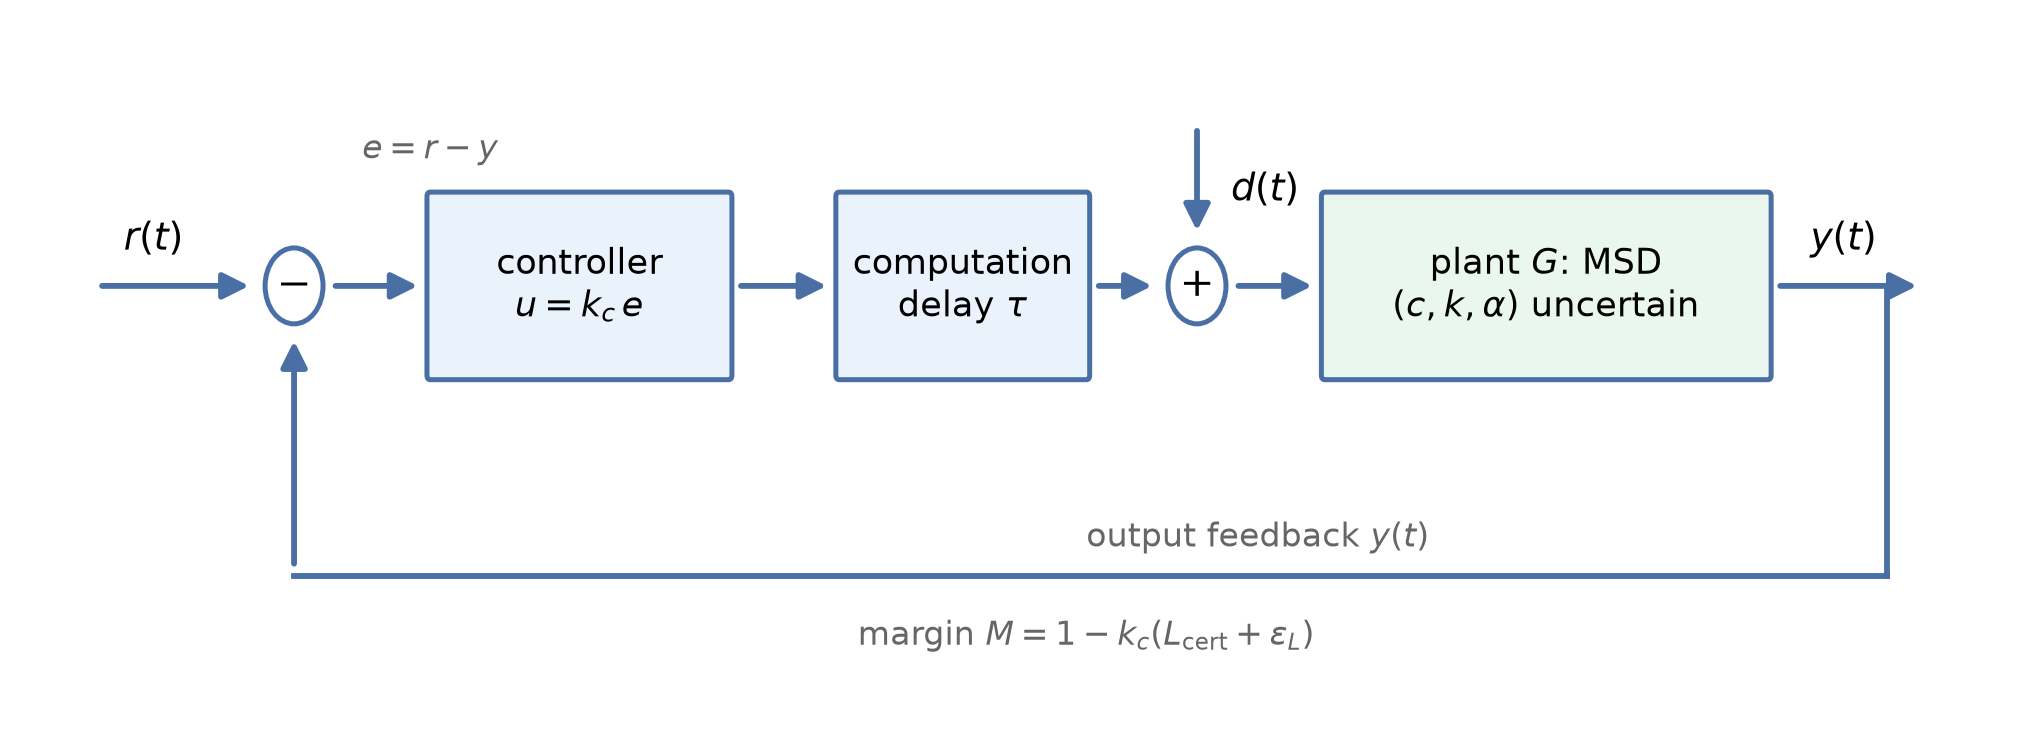
\includegraphics[width=0.85\textwidth]{fig2_loop.png}
\caption{Closed loop under study: a static output-feedback controller with a
computation delay $\tau$ in the loop, applied to the parameter-uncertain MSD
plant. The admissible gain is sized by the small-gain margin
$M=1-k_c(\Lhat+\epsL)$ built on the certificate chain of
Fig.~\ref{fig:framework}. Panel~(a) of Fig.~\ref{fig:margin} corresponds to
the smallest delay simulated (one step, $1$\,ms) and E6-B to
$\tau=50$--$200$\,ms. Theorem~\ref{thm:sg} is stated for the delay-free
interconnection; the delays simulated here fall outside its assumptions.}
\label{fig:loop}
\end{figure}

\begin{theorem}[Finite-gain robust stability]\label{thm:sg}
Assume $G$ and $C$ are causal, finite-gain, well-posed, and that the loop
keeps all signals in the working domain $\mathcal{D}$ on which
Proposition~\ref{prop:gain} holds. If
\begin{equation}
  \LC\,(\Lhat+\epsL)\;<\;1,
  \label{eq:sg}
\end{equation}
then the closed loop is finite-gain robustly stable, with the explicit
gain bound
\begin{equation}
  \|y\|_{\Ltwo}\;\le\;
  \frac{(\Lhat+\epsL)\,\LC\,\|r\|_{\Ltwo}\;+\;\|d\|_{\Ltwo}}
       {1-\LC(\Lhat+\epsL)} .
  \label{eq:sgbound}
\end{equation}
\end{theorem}
\begin{proof}
All norms are $\Ltwo([0,T])$. From the loop equations
$e=r-y$ and $u=C(e)$, the output satisfies $y=G(C(e))+d$. Since $G$ is
finite-gain with $\mathrm{Lip}(G)\le\Lhat+\epsL$
(Proposition~\ref{prop:gain}) and $C$ is $\LC$-Lipschitz,
\begin{equation*}
  \|y\|\;\le\;\mathrm{Lip}(G)\,\|C(e)\|+\|d\|
  \;\le\;(\Lhat+\epsL)\,\LC\,\|e\|+\|d\| .
\end{equation*}
The reference equation gives $\|e\|\le\|r\|+\|y\|$ (triangle inequality),
hence
\begin{equation*}
  \|y\|\;\le\;(\Lhat+\epsL)\,\LC\,\big(\|r\|+\|y\|\big)+\|d\| .
\end{equation*}
If $\LC(\Lhat+\epsL)<1$, the coefficient multiplying $\|y\|$ on the
right-hand side is strictly smaller than $1$; subtracting that term and
dividing yields \eqref{eq:sgbound}, finite for every
$(r,d)\in\Ltwo\times\Ltwo$ (well-posedness --- existence and uniqueness of
the closed-loop signals --- is hypothesised).
This two-step substitution is the standard small-gain derivation
\citep{desoer1975feedback}; the only new element is the hypothesis
replacement $\mathrm{Lip}(G)\le\Lhat+\epsL$.
\end{proof}

\begin{remark}[What is and is not claimed]\label{rem:claim}
Equation~\eqref{eq:sg} is a \emph{sufficient} condition yielding
finite-gain robust stability under the stated assumptions; it does not claim
global asymptotic stability of the origin, nor does $M\ge0$ exhaust the
stability boundary of the true nonlinear loop (the sweep experiment in the Numerical Experiments section).
A further caveat delimits the claim's strength: because $\hat\epsL$ is a
sampled \emph{lower} bound (Remark~\ref{rem:epsL}), the calibrated
quantity $\Lhat+\hat\epsL$ may under-estimate the true plant gain, in
which case \eqref{eq:sg} may fail to hold for the true loop --- the
closed-loop guarantee is \emph{empirically calibrated}, not formally
certified. The safety-factor variant prices this hedge explicitly:
inflating $\hat\epsL$ by $\gamma_s\in\{2,5,10\}$ lowers the admissible
gain from $0.241$ to $\{0.237,0.227,0.212\}$ --- at most a $12\%$
concession (Remark~\ref{rem:epsL}). Because the inflated quantity still
does not bound $\mathrm{Lip}(E)$ from above, the safety factor reduces
exposure without restoring a formal guarantee: the closed-loop statements
of this paper are heuristic design rules, and the simulation evidence in the Numerical Experiments section supports their \emph{predictive} value rather
than their formal validity. Only the model-gain statement
$\mathrm{Lip}(\Ghat)\le\Lhat$ is certified.
\end{remark}

% ---------------------------------------------------------------------
\section{Numerical Experiments}\label{sec:experiments}

\subsection{Setup}
\textbf{Plant.} Nonlinear mass--spring--damper system with parameter
uncertainty,
$q''+c\,q'+k\,q+\alpha q^3=u+d$,
$c\in[0.4,0.8]$, $k\in[0.8,1.2]$, $\alpha\in[0.5,1.2]$; full identification
benchmarks on a Duffing oscillator and a nonlinear pendulum (E8). Uncertainty
enters the \emph{data} (parameters are drawn over the box) and the a priori
analysis (Proposition~\ref{prop:apriori} holds for the whole box); the
a posteriori residual estimate, the plant-gain estimate, and the closed-loop
sweeps of E6-A and E6-B are evaluated at the nominal parameter vector
$(c,k,\alpha)=(0.6,1.0,0.85)$ at the box centre, with E6-C extending the
closed-loop check to all eight corners. \textbf{Data.} Inputs
$u(t)=\sum_{i=1}^{3}a_i\sin(2\pi f_i t+\varphi_i)$,
$a_i\sim\mathcal{U}(-1,1)$, $f_i\sim\mathcal{U}(0.2,2)$\,Hz; trajectories
integrated by RK4 ($\Delta t_{\mathrm{sim}}=10^{-3}$\,s), sampled at $N=64$
points on $[0,T]$, $T=2$\,s; 512 training / 128 in-distribution test / 128
parameter-OOD test ($\alpha\in[1.2,1.5]$) samples for the shared E1
protocol, plus a dedicated 512-sample parameter-OOD set used by E2 as an
independent robustness check.
\textbf{Training.} Adam, lr $10^{-3}$, batch 64, 100 epochs, 5 seeds;
$\lambda_{\mathrm{dyn}}=0.1$, $\lambda_{\mathrm{lip}}=1$, $\Ltarget=5$;
sensitivities to $\Ltarget$ and $\lambda_{\mathrm{lip}}$ are quantified in
E7 and to $\lambda_{\mathrm{dyn}}$ in E5.
All models share the $\sqrt{\Delta t}$ input representation where applicable;
the baselines are MLP, LSTM, Transformer, and FNO~\citep{li2021fno}.
RMSE is the root-mean-square error over all $N$ sample points and test
samples; identification and OOD metrics use $T=2$\,s windows, while E9 uses
the same definition on $4$\,s and $6$\,s trajectories, so the two are not
interchangeable.
\textbf{Baseline fairness.} Every model shares the identical protocol
(optimizer, schedule, batch size, epochs, seeds, data splits), so no baseline
is disadvantaged. The FNO in particular is given above-default
capacity---width $48$ (vs.\ $32$), $12$ Fourier modes, $4$ layers, $123$k
parameters---and converges stably (ID RMSE std $0.0009$,
Table~\ref{tab:e1}); its larger error is thus
capacity-matched rather than an optimization artifact, partly reflecting
spectral truncation and FNOs' tuning for resolution
transfer rather than a fixed grid. The point at stake is
architecture-independent: \emph{no} accuracy number yields a
computable gain certificate for FNO, whereas the proposed certificate holds by
construction.

\textbf{Experiment map and certificate provenance.}
Table~\ref{tab:emap} maps each experiment to its purpose and to the
provenance of the certificate values $\Lhat$ it reports. Each section
analyzes its \emph{own} runs: per-section $\Lhat$ values differ by design and
are never transferred between experiments. Throughout, mean$\pm$std denotes the
sample standard deviation over the stated seeds.

\begin{table}[t]
\centering\small
\caption{Experiment map. The per-section $\Lhat$ values differ by design
(different seeds and configurations) and are never transferred between
experiments.}
\label{tab:emap}
\begin{tabular}{llp{5.4cm}}
\toprule
Exp. & Purpose & $\Lhat$ provenance \\
\midrule
E1 & Identification accuracy & per-run (demonstration run of Fig.~\ref{fig:training}: 3.92) \\
E2 & Parameter-OOD regime & per-run (OOD columns of Table~\ref{tab:e1}; dedicated 512-sample set: 4.16) \\
E3 & Sensitivity vs.\ certificate & 3.89$\pm$0.21 (5 seeds) \\
E4 & Input-noise robustness & -- \\
E10 & Binding-target closed loop and transfer & $1.97\pm0.14$ / $1.97\pm0.15$ / $1.70\pm0.37$ (MSD/Duffing/pendulum, 5 seeds) \\
E5 & Ablation; $\lambda_{\mathrm{dyn}}$ sweep & 4.06$\pm$0.37 (config B), 4.03$\pm$0.31 (config D); 5 seeds \\
E6-A/B & Closed-loop small-gain & 3.68 (single design run, $\hat\epsL=0.056$) \\
E6-C & Parameter-box corners & 3.93$\pm$0.25 (5 seeds; $\hat\epsL$ re-estimated per corner) \\
E7 & Certificate--accuracy trade-off & 1.53--4.00 (function of $\Ltarget$; 5 seeds each) \\
E8 & Cross-system transfer & 4.12$\pm$0.35 (Duffing), 3.37$\pm$0.08 (pendulum) \\
E9 & Long-horizon rollout & -- \\
M3 & Certificate tightness (Frobenius vs.\ spectral) & 3.91$\pm$0.32 $\to$ 3.31$\pm$0.29 (5 seeds) \\
\bottomrule
\end{tabular}
\end{table}

\begin{table}[t]
\centering\small
\caption{Identification performance on the parameter-uncertain MSD system
(mean $\pm$ std over 5 seeds). OOD: $\alpha\in[1.2,1.5]$ not seen in training.}
\label{tab:e1}
\begin{tabular}{lrrrr}
\toprule
Model & \#Params & ID RMSE & OOD RMSE & Infer (ms) \\
\midrule
MLP          & 98{,}880  & 0.0102$\pm$0.0004 & 0.0112$\pm$0.0002 & 0.0003 \\
LSTM         & 199{,}297 & 0.0157$\pm$0.0045 & 0.0211$\pm$0.0039 & 0.0030 \\
Transformer  & 267{,}841 & 0.0306$\pm$0.0062 & 0.0360$\pm$0.0061 & 0.0071 \\
FNO          & 123{,}297 & 0.0360$\pm$0.0009 & 0.0481$\pm$0.0020 & 0.0010 \\
DeepONet     & 181{,}696 & 0.0120$\pm$0.0015 & 0.0135$\pm$0.0008 & 0.0002 \\
\textbf{LC-DeepONet} & 181{,}696 & \textbf{0.0112$\pm$0.0010} & \textbf{0.0128$\pm$0.0011} & 0.0002 \\
\bottomrule
\end{tabular}
\end{table}

\subsection{E1--E2: Identification accuracy and parameter OOD}
Table~\ref{tab:e1} shows that the constraint does not sacrifice accuracy:
LC-DeepONet attains a lower mean RMSE than the unconstrained DeepONet in both
regimes with smaller per-seed variance; the remaining gap to the best
overall baseline (MLP, $0.0102\pm0.0004$) is $0.0009$, just below the
LC-DeepONet seed spread ($0.0010$). At the
default target the penalty is inactive (Proposed Method section), so this
compares two identically parameterised networks; the binding-target evidence
is E7, where a $62\%$ tighter certificate leaves the error within one seed
standard deviation. On the parameter-OOD regime ($\alpha\in[1.2,1.5]$, 5 seeds) the two generalize
comparably: the 128-sample split of the E1 protocol slightly favours the
constrained model ($0.0128\pm0.0011$ vs.\ $0.0135\pm0.0008$), while the
dedicated 512-sample set of E2 makes them statistically indistinguishable
($0.0120\pm0.0013$ vs.\ $0.0116\pm0.0008$, \texttt{e2\_ood.csv}), the ordering
reversing between two independent test sets. We therefore report
\emph{no measurable generalization penalty}, not a generalization gain, and
the value of the certificate is a stability-relevant gain bound at essentially
zero accuracy cost. Fig.~\ref{fig:training} shows the training dynamics (equal
convergence rate, surrogate below target throughout), and
Fig.~\ref{fig:accuracy} inspects the \emph{character} of the error on the
worst-case test trajectory and summarizes ID/OOD across all baselines.

\begin{figure}[t]
\centering
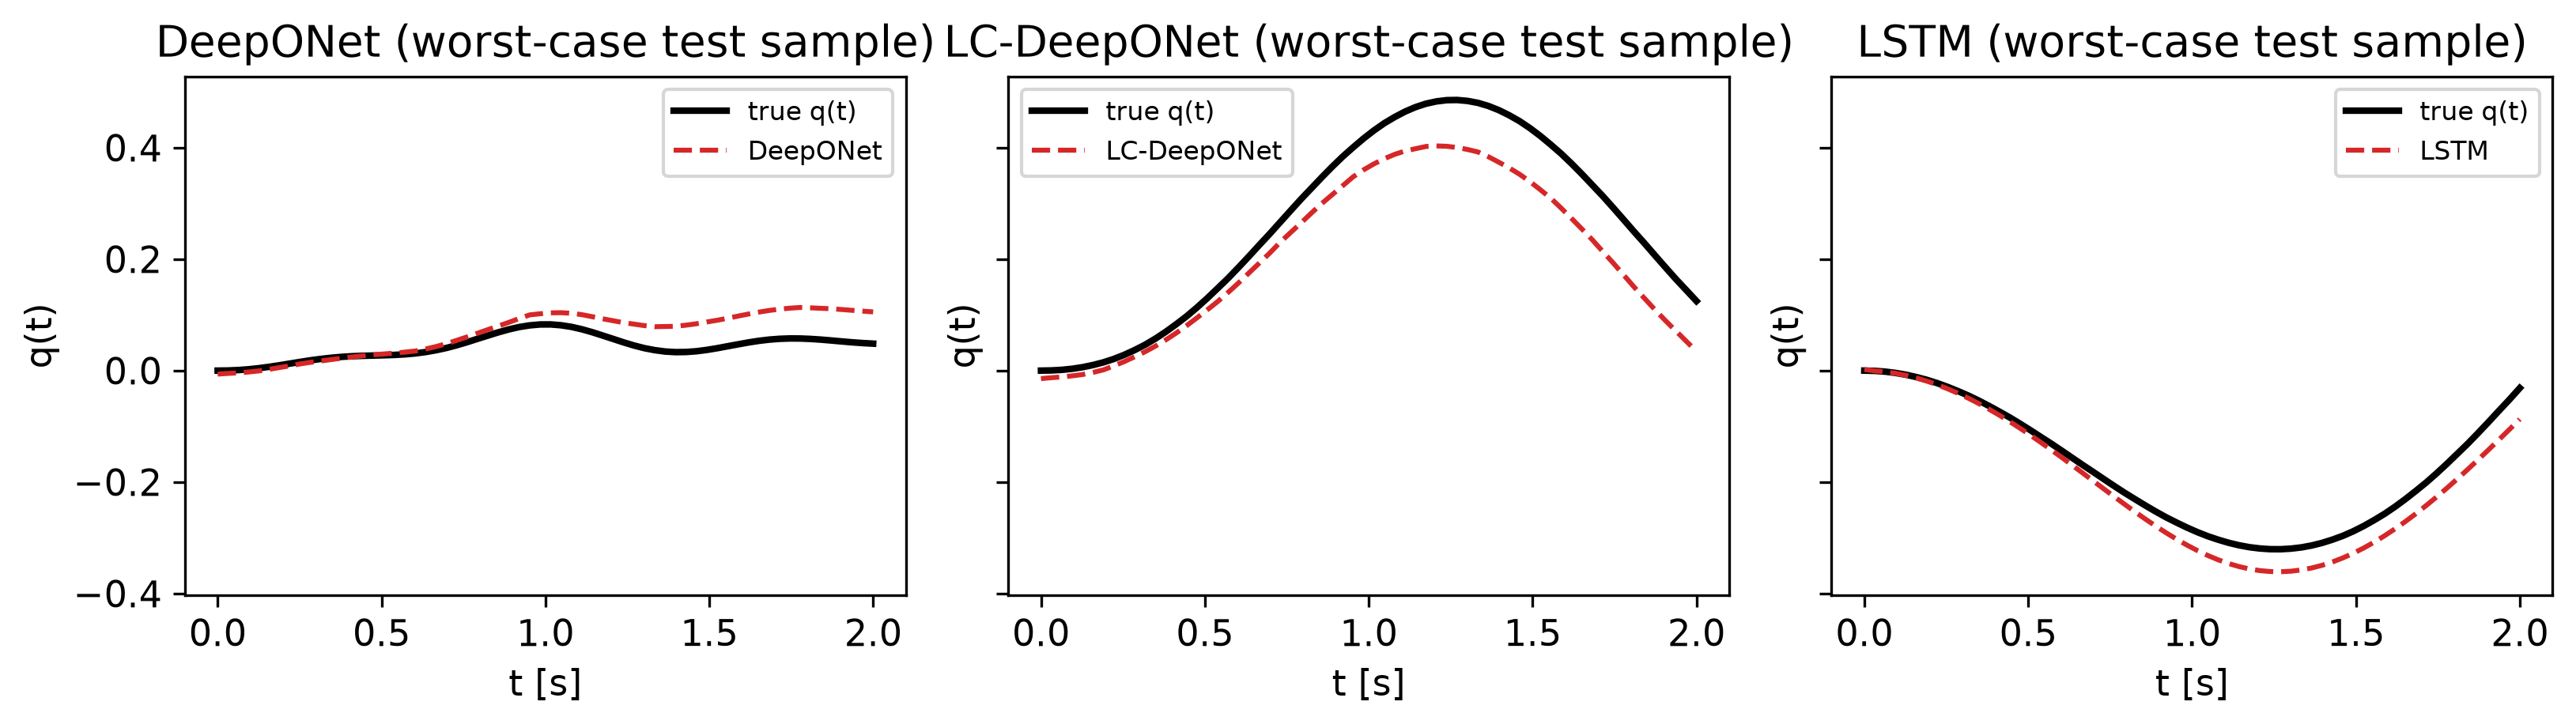
\includegraphics[width=\textwidth]{fig4_identification.png}\\[4pt]
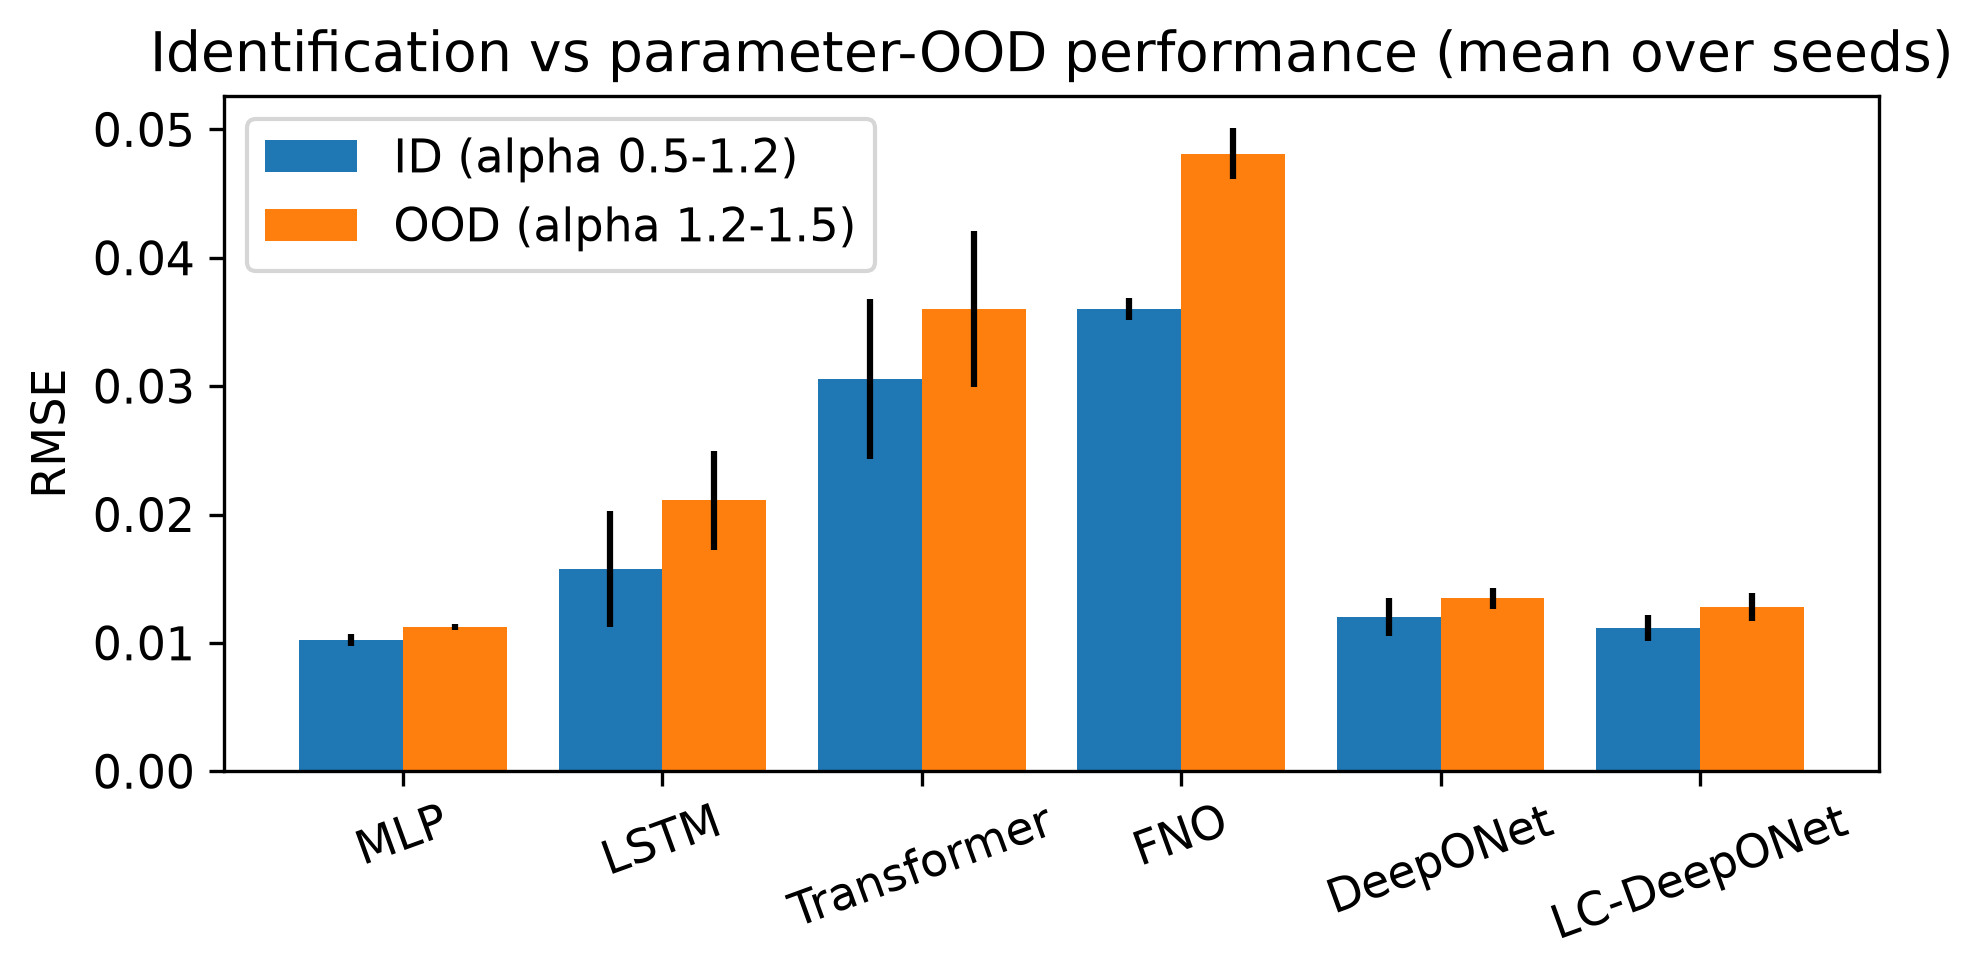
\includegraphics[width=0.8\textwidth]{fig5_ood.png}
\caption{Identification accuracy. (a)~Worst-case in-distribution test
sample (largest per-sample error) for the unconstrained DeepONet,
LC-DeepONet and the LSTM baseline: the purpose is to inspect where the
largest errors come from. All three models follow the reference waveform,
and on this hardest sample the residual is dominated by a phase lag
combined with a small amplitude deviation rather than by a large amplitude
excursion, which corroborates at the trajectory level the aggregate
comparison of Table~\ref{tab:e1}. The LSTM is included as a representative
recurrent baseline, and panel~(b) carries the comparison for all six
models. (b)~ID vs.\ parameter-OOD RMSE (mean $\pm$ std over
5 seeds): the Lipschitz constraint costs no measurable generalization on
the OOD regime.}
\label{fig:accuracy}
\end{figure}

\begin{figure}[t]
\centering
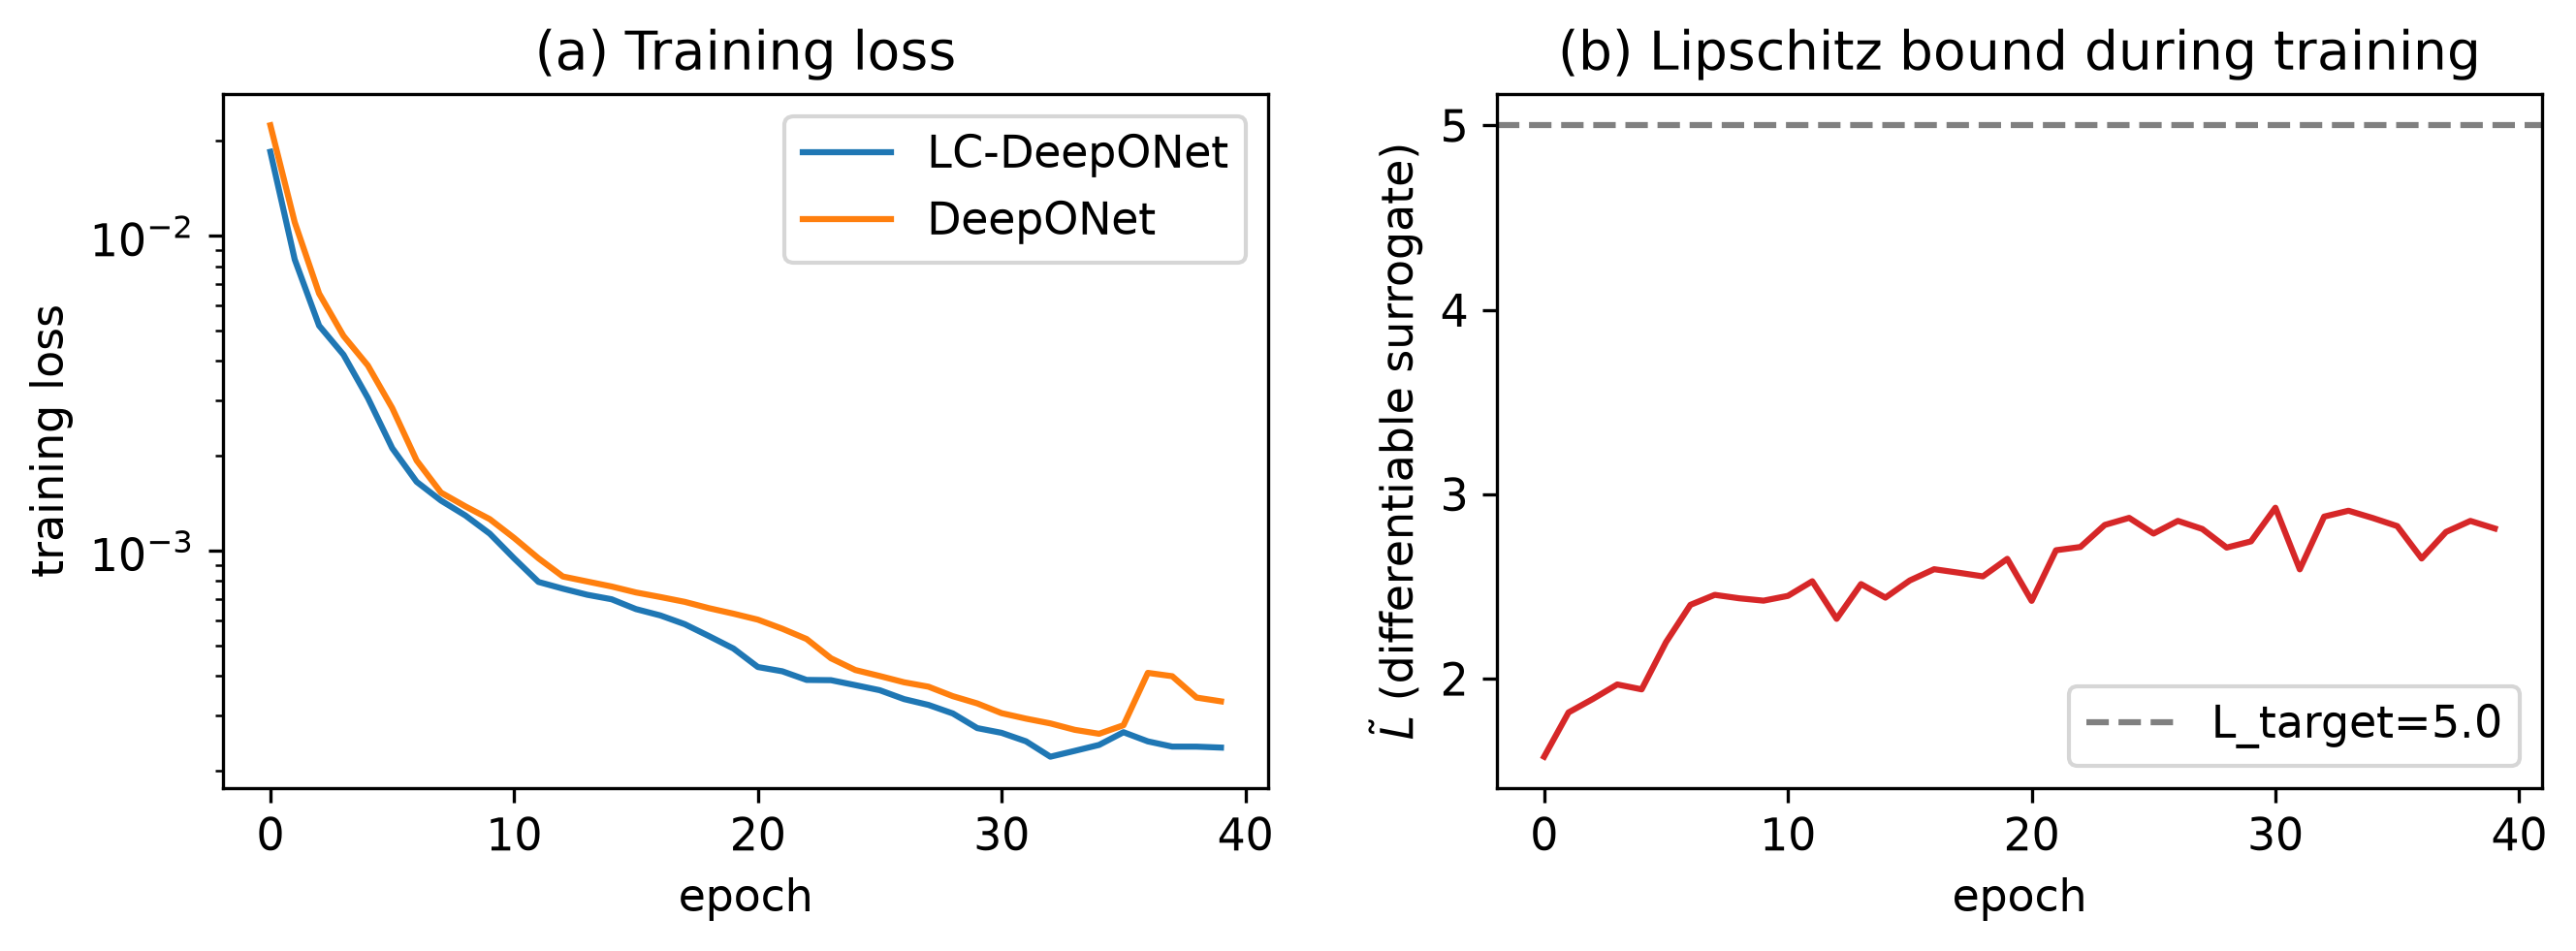
\includegraphics[width=0.9\textwidth]{fig3_training_lipschitz.png}
\caption{Training dynamics. (a)~Training loss of LC-DeepONet versus the
unconstrained DeepONet: the spectral penalty costs no convergence speed or
final accuracy. (b)~The differentiable surrogate
$\tilde L=(\prod_i s_i)\,C_{\mathrm{T}}$ (power iteration on the branch
weights) remains below the target $L_{\mathrm{target}}=5$ throughout
training, so the safeguard remains inactive in this demonstration;
the demonstration run shown here ends at $\Lhat=3.92$ --- each experiment
reports its own runs' certificates (Table~\ref{tab:emap}).}
\label{fig:training}
\end{figure}

\subsection{E3: Empirical sensitivity vs.\ certificate}
Over five training seeds, the certified bound ($\Lhat=3.89\pm0.21$,
evaluated exactly via SVD after training) encloses the empirical
input-perturbation sensitivity of the learned operator
($S_{\mathrm{emp}}=0.265\pm0.012$) with an order-of-magnitude margin;
the residual Lipschitz estimate is $\hat\epsL=0.040\pm0.008$, giving
the empirically calibrated plant bound $\Lhat+\hat\epsL=3.93\pm0.22$.
For comparison, the unconstrained baselines possess no computable
certificate at all; the FNO in particular exhibits an empirical sensitivity
of $2.55\pm0.73$ (Fig.~\ref{fig:sensitivity}).

\begin{figure}[t]
\centering
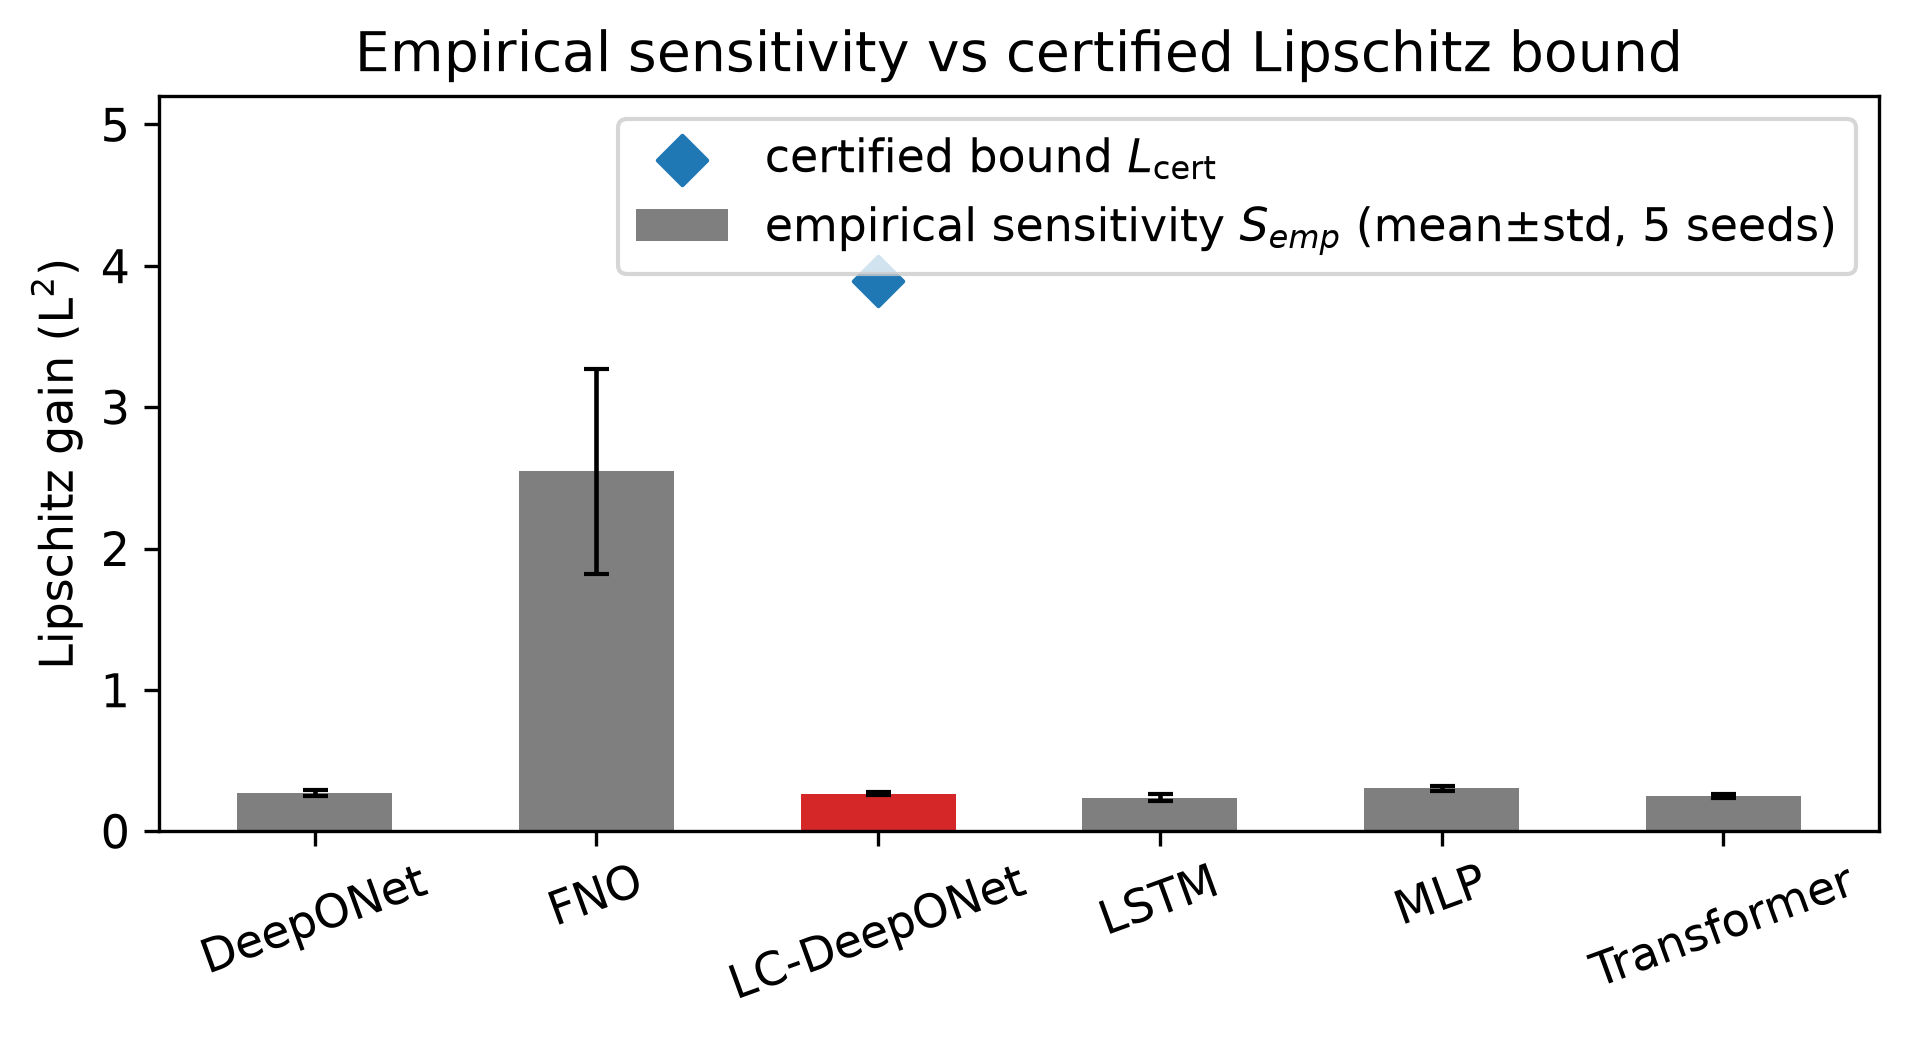
\includegraphics[width=0.8\textwidth]{fig7_sensitivity_vs_certificate.png}
\caption{Empirical input-perturbation sensitivity $S_{\mathrm{emp}}$ vs.\
the certified Lipschitz bound $\Lhat$ (E3). Only LC-DeepONet possesses a
computable certificate; the FNO baseline's large sensitivity would have
been exposed by it a priori.}
\label{fig:sensitivity}
\end{figure}

On these five seeds the other architectures reach $S_{\mathrm{emp}}=0.30\pm0.02$ (MLP),
$0.24\pm0.02$ (LSTM), $0.25\pm0.02$ (Transformer) and $0.27\pm0.02$
(DeepONet) against $0.265\pm0.012$ for LC-DeepONet
(\texttt{e3b\_sensitivity\_per\_seed.csv}), so LC-DeepONet is not the least
sensitive model: its advantage is a \emph{computable upper bound}, not a
smaller measured sensitivity. The FNO is singled out only because its
sensitivity ($2.55\pm0.73$) is an order of magnitude above the rest, which
makes the absence of any bound for it the most conspicuous.

\subsection{E4: Robustness to test-time input noise}
The models are trained on clean data only and evaluated on the ID test set
with Gaussian input noise of level $\ell\,\|u\|_\infty$ added at test time,
$\ell\in\{1,3,5,10\}\%$ (mean $\pm$ std over 5 training seeds, with the
noise realizations fixed across models; Fig.~\ref{fig:noise}). The protocol
isolates operator-level disturbance amplification: nothing in training
prepares the model for the perturbation, so the RMSE growth directly
reflects the input--output gain that E3 measured adversarially.
LC-DeepONet degrades gracefully from $0.0126\pm0.0013$ at $1\%$ noise to
$0.0254\pm0.0012$ at $10\%$, at or slightly below the unconstrained DeepONet
at every level ($0.0146\pm0.0024\to0.0257\pm0.0016$; the largest gap, $0.0020$
at $1\%$ noise, is below the seed standard deviation $0.0024$), whereas the
FNO baseline degrades from $0.0393\pm0.0013$ to $0.0961\pm0.0055$, the
steepest of the six: its error exceeds the DeepONet family by an order of
magnitude at every level, far beyond the seed variability (the Transformer is
the only other baseline separated from LC-DeepONet by more than one seed
standard deviation at every level). The correspondence with the measured
sensitivity of E3 holds only at the top of the ranking --- the FNO, with ten
times any other model's sensitivity, is also the least robust; among the
remaining five it is weak and we read it as qualitative.

\begin{figure}[t]
\centering
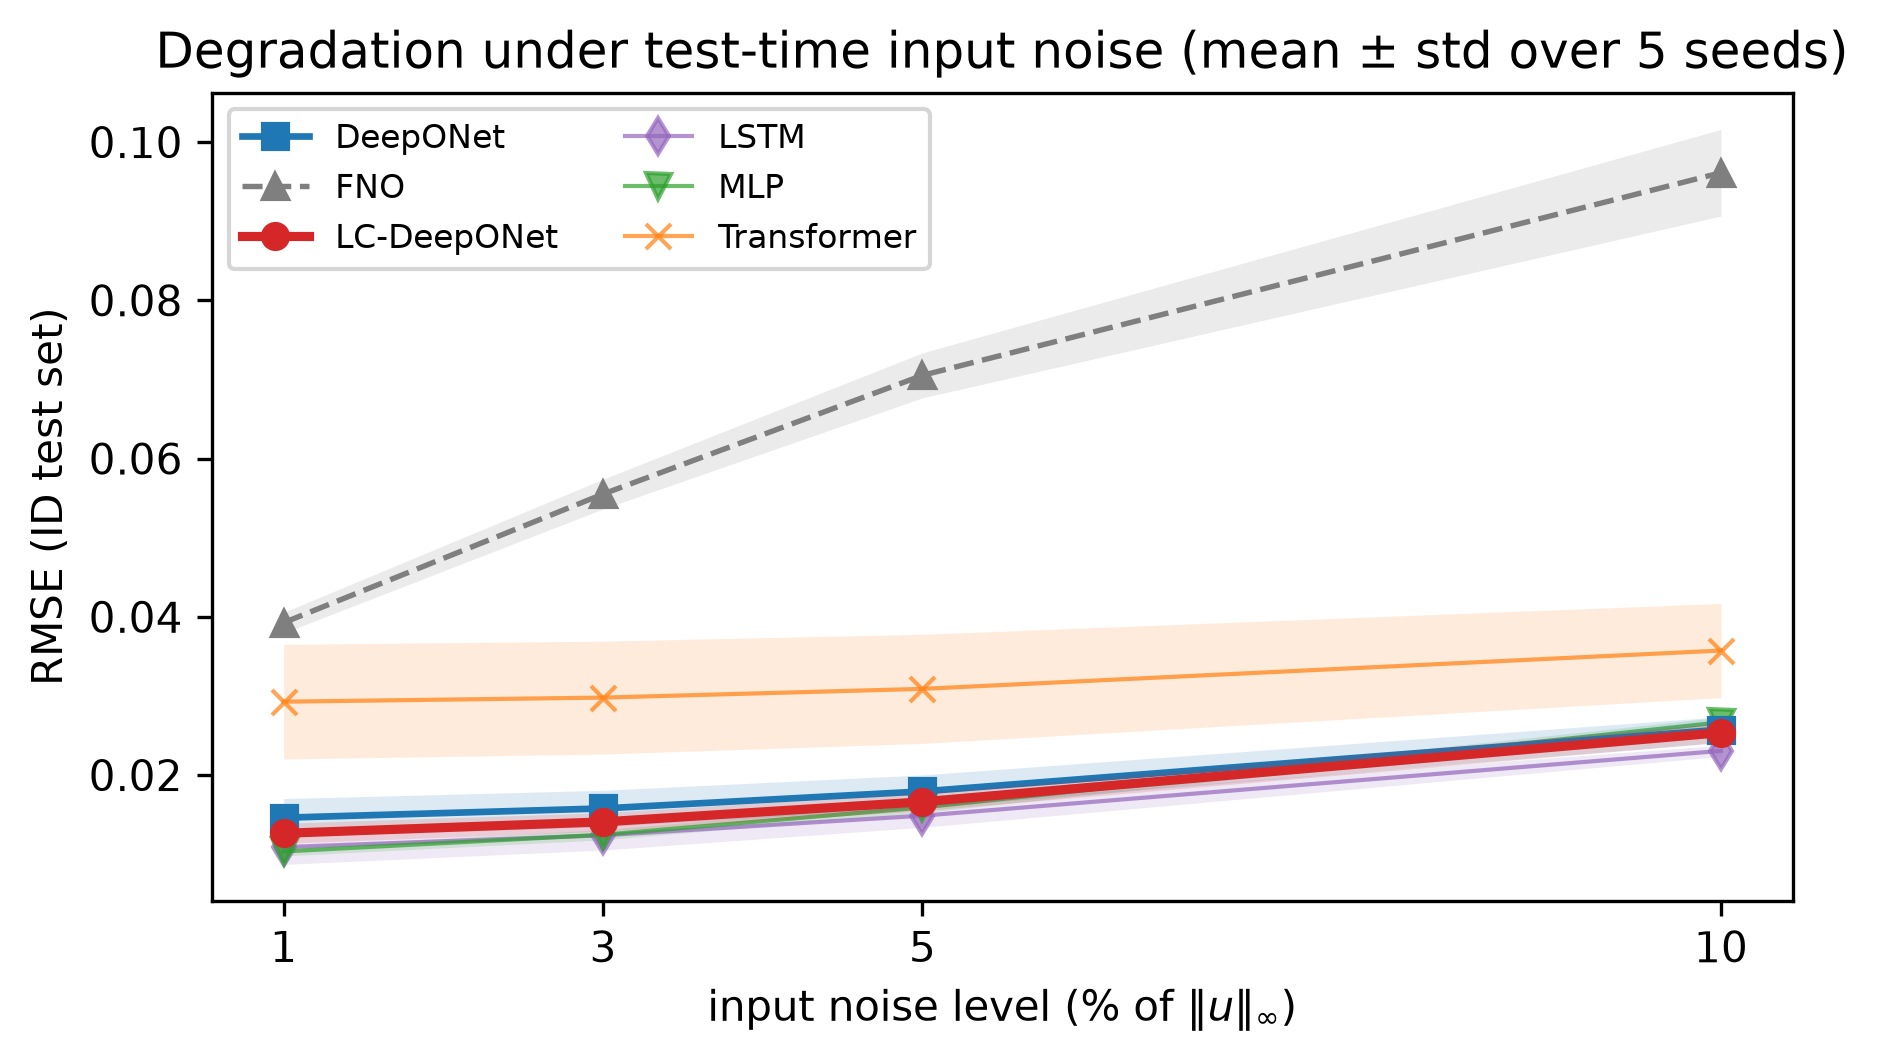
\includegraphics[width=0.8\textwidth]{fig6_noise.png}
\caption{RMSE under test-time input noise (clean-trained models, ID test
set, mean over five training seeds). The Lipschitz-constrained model degrades as gracefully
as its unconstrained counterpart; the FNO baseline, whose measured
operator sensitivity is an order of magnitude larger, amplifies the
perturbation accordingly.}
\label{fig:noise}
\end{figure}

\subsection{E5: Ablation and the role of the dynamic loss}
With a fixed LC-DeepONet backbone, four configurations isolate the two
additions, five seeds each (Table~\ref{tab:e5}). The full method (D) is best
in both ID and OOD accuracy ($0.0116\pm0.0007$, $0.0129\pm0.0010$). The
$+$Lip configuration (B) does not improve on the bare backbone (A) --- its
standalone value is the certificate it supplies ($\Lhat=4.06\pm0.37$) --- and
Since the hinge term is identically zero at $\Ltarget=5$ (E7), no active
penalty differs between B and A, which share one architecture; at $n=5$ the
arm-to-arm spread (ID std $0.0024$ vs.\ $0.0007$) is therefore read as
seed-level variability, not as a property of the constraint. The role of the
dynamic loss is \emph{stabilization} rather than extra accuracy: the full
method returns to the baseline level and the dynamic loss alone (C) lies
between the two.

A five-seed sweep over $\lambda_{\mathrm{dyn}}\in\{0,0.01,0.1,1\}$
(Table~\ref{tab:e5lam}) supports the same reading: intermediate weights give
the best and most stable ID/OOD errors, $\lambda_{\mathrm{dyn}}=0$ shows the
largest seed variance, $\lambda_{\mathrm{dyn}}=1$ is mildly
counterproductive, and the long-horizon (4\,s) RMSE is essentially identical
throughout.

\begin{table}[t]
\centering\small
\caption{Ablation on $\{$Lipschitz penalty$\}\times\{$dynamic loss$\}$
(mean $\pm$ std over 5 seeds). All four arms share the LC-DeepONet backbone;
A disables both additions, and both switches act on the loss only.}
\label{tab:e5}
\begin{tabular}{lcccrc}
\toprule
Config & Lip & Dyn & ID RMSE & OOD RMSE & $\Lhat$ \\
\midrule
A (backbone only) & -- & -- & 0.0118$\pm$0.0007 & 0.0137$\pm$0.0005 & -- \\
B (+Lip)          & \checkmark & -- & 0.0136$\pm$0.0024 & 0.0148$\pm$0.0023 & 4.06$\pm$0.37 \\
C (+Dyn)          & -- & \checkmark & 0.0127$\pm$0.0042 & 0.0140$\pm$0.0041 & -- \\
D (full LC)       & \checkmark & \checkmark & \textbf{0.0116$\pm$0.0007} & \textbf{0.0129$\pm$0.0010} & 4.03$\pm$0.31 \\
\bottomrule
\end{tabular}
\end{table}

\begin{table}[t]
\centering\small
\caption{Sensitivity to the dynamic-loss weight $\lambda_{\mathrm{dyn}}$
(mean $\pm$ std over 5 seeds). RMSE(4\,s) is the root-mean-square error over
the whole 4\,s horizon, computed on a test set generated for this sweep: it
uses the same metric as E9 but a different data draw and a different
configuration, so its absolute level ($0.1023$--$0.1026$) is not comparable
with the E9 numbers and only its variation within the sweep should be read.
That variation is essentially flat (max deviation $0.3\%$), so the column is
not intended to resolve differences between the weights.}
\label{tab:e5lam}
\begin{tabular}{lccc}
\toprule
$\lambda_{\mathrm{dyn}}$ & ID RMSE & OOD RMSE & RMSE(4\,s) \\
\midrule
0    & 0.0130$\pm$0.0037 & 0.0148$\pm$0.0041 & 0.1026$\pm$0.0010 \\
0.01 & 0.0119$\pm$0.0010 & \textbf{0.0129$\pm$0.0009} & 0.1025$\pm$0.0006 \\
0.1  & \textbf{0.0119$\pm$0.0017} & 0.0135$\pm$0.0010 & 0.1023$\pm$0.0004 \\
1    & 0.0127$\pm$0.0024 & 0.0138$\pm$0.0019 & 0.1023$\pm$0.0007 \\
\bottomrule
\end{tabular}
\end{table}

\subsection{E6: Closed loop and the small-gain margin}
The design uses the empirically calibrated bound $\Lhat+\hat\epsL=3.73$ from
the single design run (seed $42$; certificate $\Lhat=3.678$,
$\hat\epsL=0.056$, all quantities in
\texttt{results/e6\_design\_provenance.csv}), giving
$k_c^{\mathrm{safe}}=0.9/(\Lhat+\hat\epsL)=0.241$ and margin $M=0.1>0$.
Four groups of closed-loop experiments are run on the \emph{true} plant.

\emph{Scope.} As stated in the Numerical Experiments section, these quantities are
calibrated at the nominal vector; E6-C below re-estimates them at all eight box
corners, and whole-box coverage is provided analytically by
Proposition~\ref{prop:apriori} at roughly $2.8\times$ the conservatism
(Remark~\ref{rem:price}).

\emph{E6-A (no intentional delay; certificate-consistent).} The controller
is $u=k_c(r-y)$ updated every step, i.e.\ a one-step ($1$\,ms) lag, two orders
of magnitude below the closed-loop bandwidth ($\approx0.5$\,Hz) and the
configuration closest to the delay-free interconnection assumed by the
analysis. Sweeping $k_c$ over $0.25\times$--$128\times$ of
$k_c^{\mathrm{safe}}$ (Fig.~\ref{fig:margin}a) shows: (i) for $M>0$ the
tracking error decreases monotonically ($0.977\to0.909$), as theory permits; (ii) for $M<0$ the condition no
longer holds and the error becomes non-monotone (it keeps decreasing to
$0.255$ around $16\times$--$32\times$, then rises to $0.51$ at $128\times$),
as does the overshoot ($1.41$ at $128\times$). No divergence occurs at any gain:
the hardening nonlinearity and dissipation preclude finite-time blow-up under
static negative feedback, so the margin predicts the loss of the
\emph{guarantee}, not of stability
(Remark~\ref{rem:claim}); Fig.~\ref{fig:marginrmse} condenses the sweep into
the margin--performance plane. (iii) Replacing the calibrated bound by an
empirical sensitivity alone is unjustified. The design run's unconstrained
DeepONet has $S_{\mathrm{emp}}=0.254$, giving
$k_c^{\mathrm{opt}}=0.9/S_{\mathrm{emp}}=3.541$ ($14.7\times$ the calibrated
gain); the E3 five-seed mean ($0.269$) and the constrained model's own
sensitivity ($0.265$) give $3.35$ and $3.40$, so the risk is not specific to
the unconstrained baseline. Either way the premise is mistaken: a sampled lower
bound on the \emph{model's} gain carries no information about the plant's
($\widehat{\mathrm{Lip}}(G)\approx0.52$ at the nominal vector); the
certificate is conservative but valid, the empirical sensitivity aggressive
and \emph{unjustified}. Judged against the plant gain rather than the model
sensitivity, the certificate design keeps $M>0$ in all five seeds, the
optimistic design in none ($M=-0.86\pm0.06$; E6-D).

\emph{E6-B (implementation delay).} Real implementations inject a computation
delay $\tau$ (infinite-dimensional and outside the stated assumptions).
Repeating the sweep with $u=k_c(r-y(t-\tau))$ for $\tau\in\{50,100,200\}$\,ms isolates
its role (Fig.~\ref{fig:margin}b): inside the calibrated region the error is
nearly delay-insensitive ($0.909$ at the one-step lag to $0.947$ at
$\tau=200$\,ms), whereas at $128\,k_c^{\mathrm{safe}}$ the tracking error
grows from $0.51$ to $1.38$, $2.82$, $2.97$ and the overshoot from $1.41$ to
$2.28$, $4.94$, $7.88$ for $\tau=50,100,200$\,ms
(Fig.~\ref{fig:margin}c,d). The margin-blessed design thus absorbs
non-idealities for which the aggressive design has no spare margin.

\emph{E6-C (parameter-box corners).} E6-C re-estimates the residual sensitivity and the
sampled plant gain at all eight corners with the same five trained models and
repeats the closed-loop comparison there (Table~\ref{tab:e6c}). The residual
estimate varies most: $\hat\epsL$ rises from $0.039$ at the centre to $0.124$
at the worst corner, a factor of $3.2$, whereas the sampled plant gain and the
total bound move only from $0.517$ to $0.587$ and from $3.96$ to $4.03$,
because the certified gain $\Lhat\approx3.9$ dominates the sum.
Consequently the calibrated bound covers the sampled plant gain at
\emph{every} corner, and the design gain is nearly insensitive to where in the
box the calibration is performed: the worst corner gives $k_c=0.222$ against
$0.227$ at the centre, a $2\%$ reduction. (The two aggregates differ by construction, and E6-D replaces
the single-seed design of E6-A/B.) All nine parameter points close stably with
essentially identical tracking error ($0.921$--$0.934$), so the design
transfers across the box rather than being tuned to one instance.

\emph{E6-D (seed-to-seed reproducibility).} Re-running the whole pipeline on
five independently trained networks reproduces the picture above:
$k_c^{\mathrm{safe}}=0.234\pm0.006$, and at every gain multiple the five
sweeps agree to within a few per cent without a single divergence
(\texttt{results/e6s\_summary.csv}); the margin survives replication rather
than depending on one draw.

\begin{table}[t]
\centering\small
\caption{Parameter-box corner check (E6-C; the same five trained models as
E6-A/B). The residual sensitivity varies most across the box, while the total
calibrated bound and the design gain are nearly invariant because the
certified model gain dominates. Every corner satisfies
$\Lhat+\hat\epsL\ge$ sampled plant gain, and every closed-loop run is stable
with essentially the same tracking error. These errors are not directly
comparable with the $0.909$ and $0.922$ of Fig.~\ref{fig:margin}: they use
the five-seed mean design gain ($k_c=0.227$ rather than $0.241$) at a
$100$\,ms delay.}
\label{tab:e6c}
\begin{tabular}{lccccc}
\toprule
Point & $\hat\epsL$ mean & $\hat\epsL$ max & sampled $\mathrm{Lip}(G)$ & $\Lhat+\hat\epsL$ & tracking error \\
\midrule
centre $(0.6,1.0,0.85)$        & 0.039 & 0.050 & 0.517 & 3.96 & 0.927 \\
worst corner $(0.4,0.8,0.5)$   & 0.105 & 0.124 & 0.587 & 4.03 & 0.921 \\
\multicolumn{1}{l}{range over the 8 corners} & 0.045--0.105 & 0.063--0.124 & 0.460--0.587 & 3.97--4.03 & 0.921--0.934 \\
\bottomrule
\end{tabular}
\end{table}

\begin{figure}[htbp]
\centering
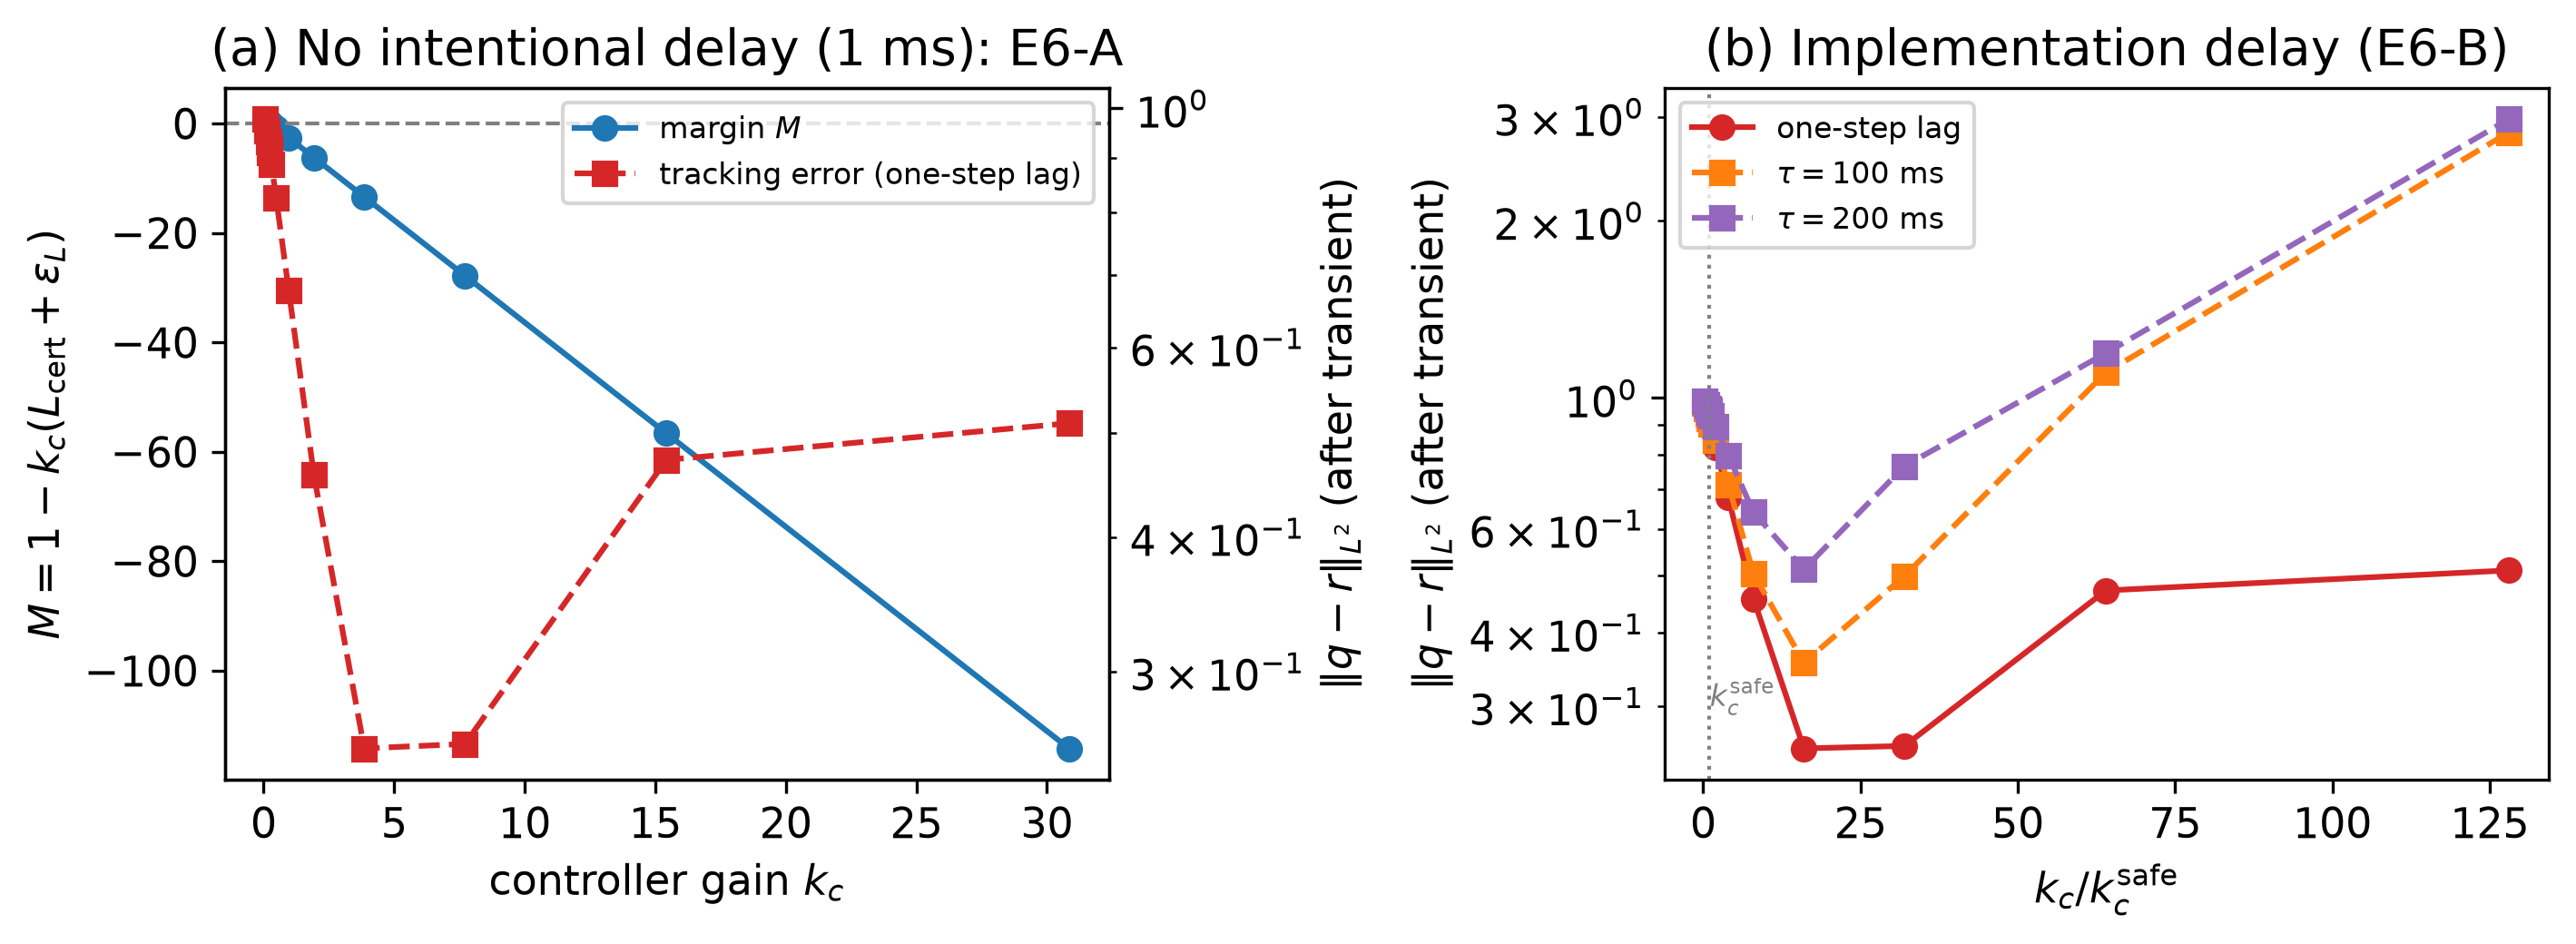
\includegraphics[width=0.92\textwidth]{fig8_smallgain_margin.png}\\[4pt]
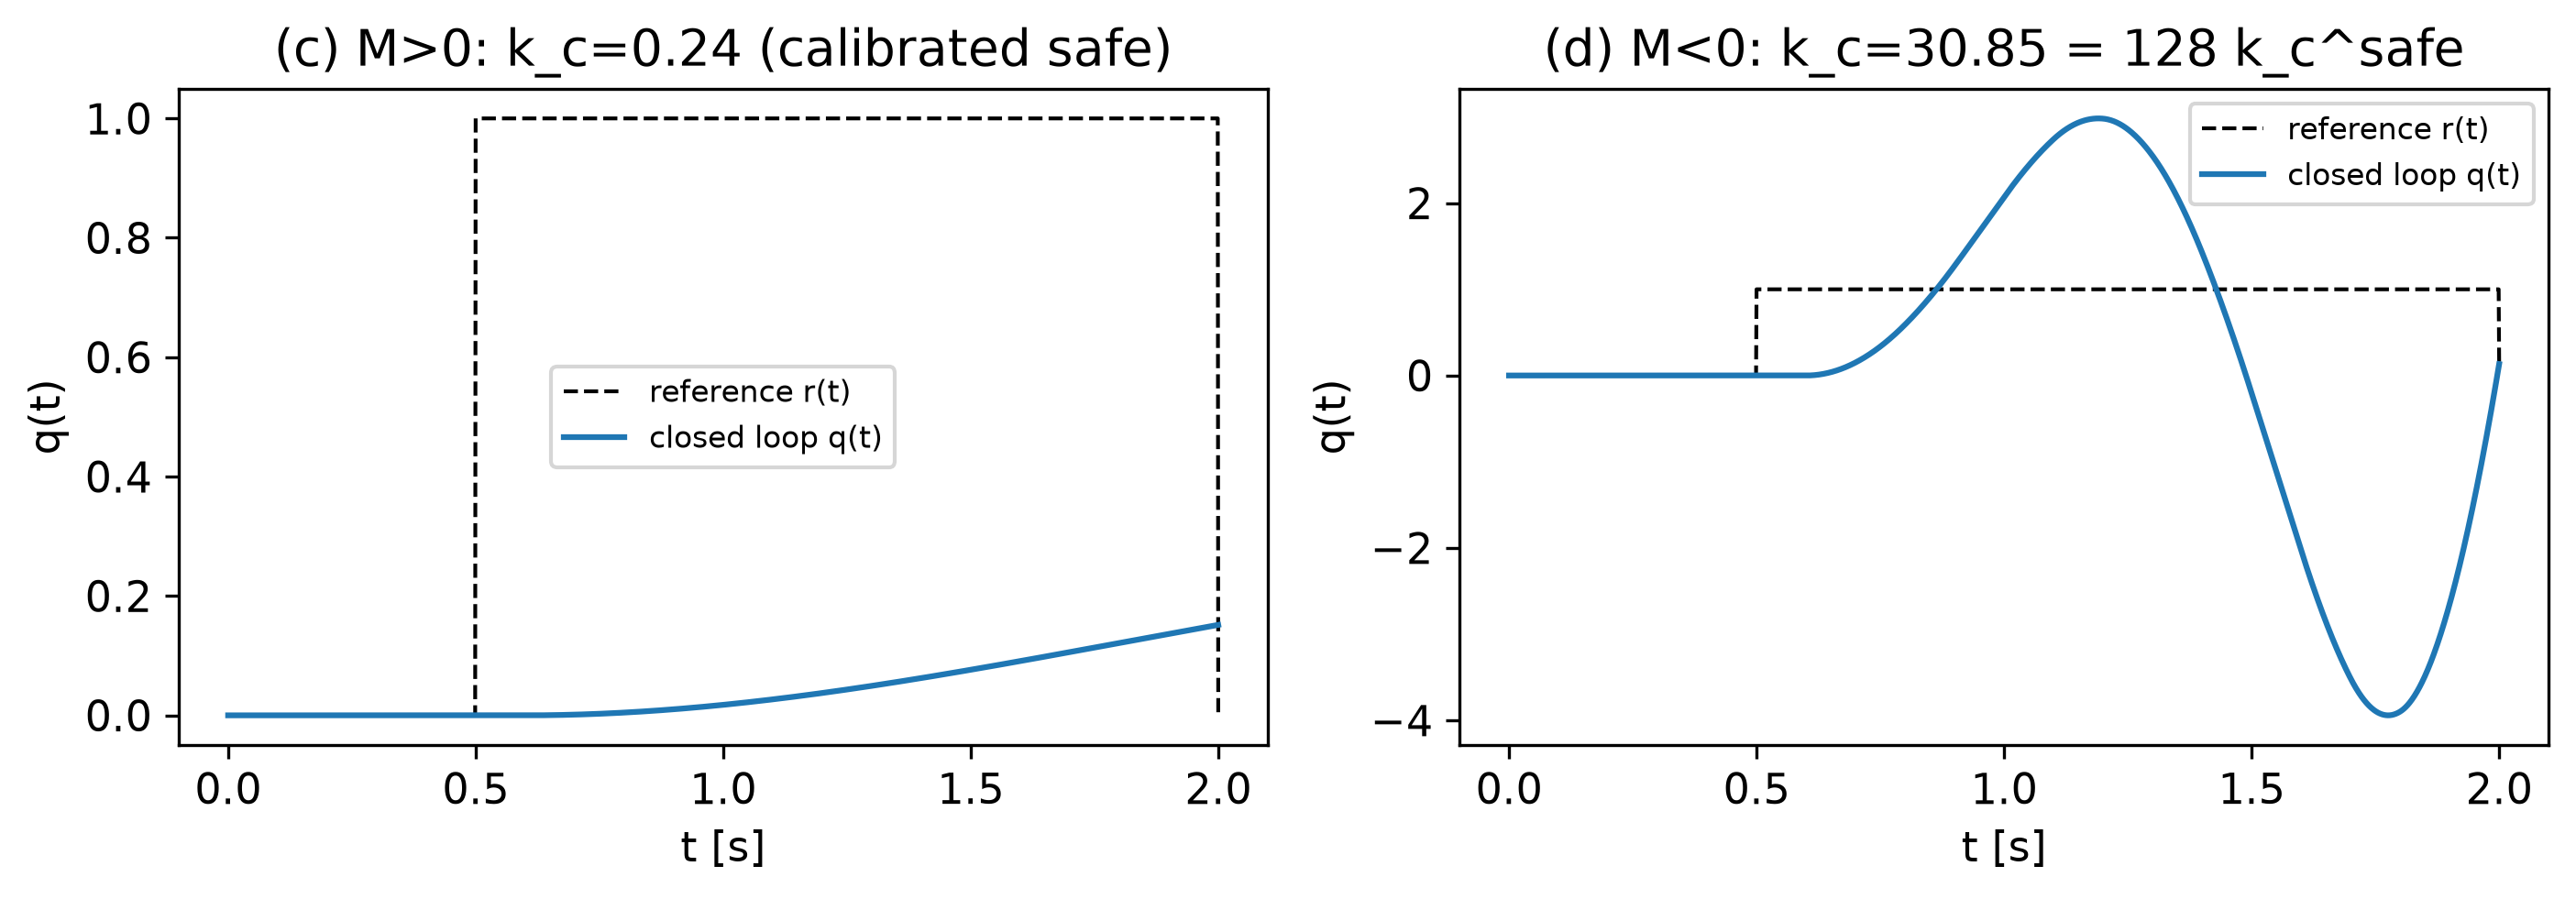
\includegraphics[width=0.92\textwidth]{fig9_closedloop.png}
\caption{Closed-loop experiments (E6). (a)~Margin sweep at a one-step
($1$\,ms) lag, the configuration closest to the delay-free interconnection
of the analysis (E6-A): margin $M=1-k_c(\Lhat+\hat\epsL)$ versus controller
gain $k_c$, crossing zero at $k_c^{\mathrm{safe}}=0.241$; the tracking error
decreases monotonically while $M>0$ and becomes non-monotone once the
calibrated condition is lost ($M<0$), with no divergence at any gain.
(b)~Implementation
delay (E6-B): tracking error versus $k_c/k_c^{\mathrm{safe}}$ for
a one-step ($1$\,ms) lag and $\tau=100,200$\,ms; the calibrated region
(dotted line at $1\times$)
is delay-insensitive, while the uncertified high-gain region is
amplified by up to $5.8\times$ ($\tau=200$\,ms, $128\times$).
(c)~Closed-loop trajectories with $\tau=100$\,ms: the calibrated design
($k_c=k_c^{\mathrm{safe}}$, $M=0.1>0$) keeps the response bounded and close
to the reference (tracking error $0.922$, against $0.909$ at the one-step
lag), with a small residual offset visible after the step.
(d)~The uncertified design ($k_c=128\,k_c^{\mathrm{safe}}$, $M<0$)
exhibits a severely degraded, oscillatory response (overshoot $4.94$):
with no spare margin, the implementation delay consumes what little
robustness the design had.}
\label{fig:margin}
\end{figure}

\begin{figure}[htbp]
\centering
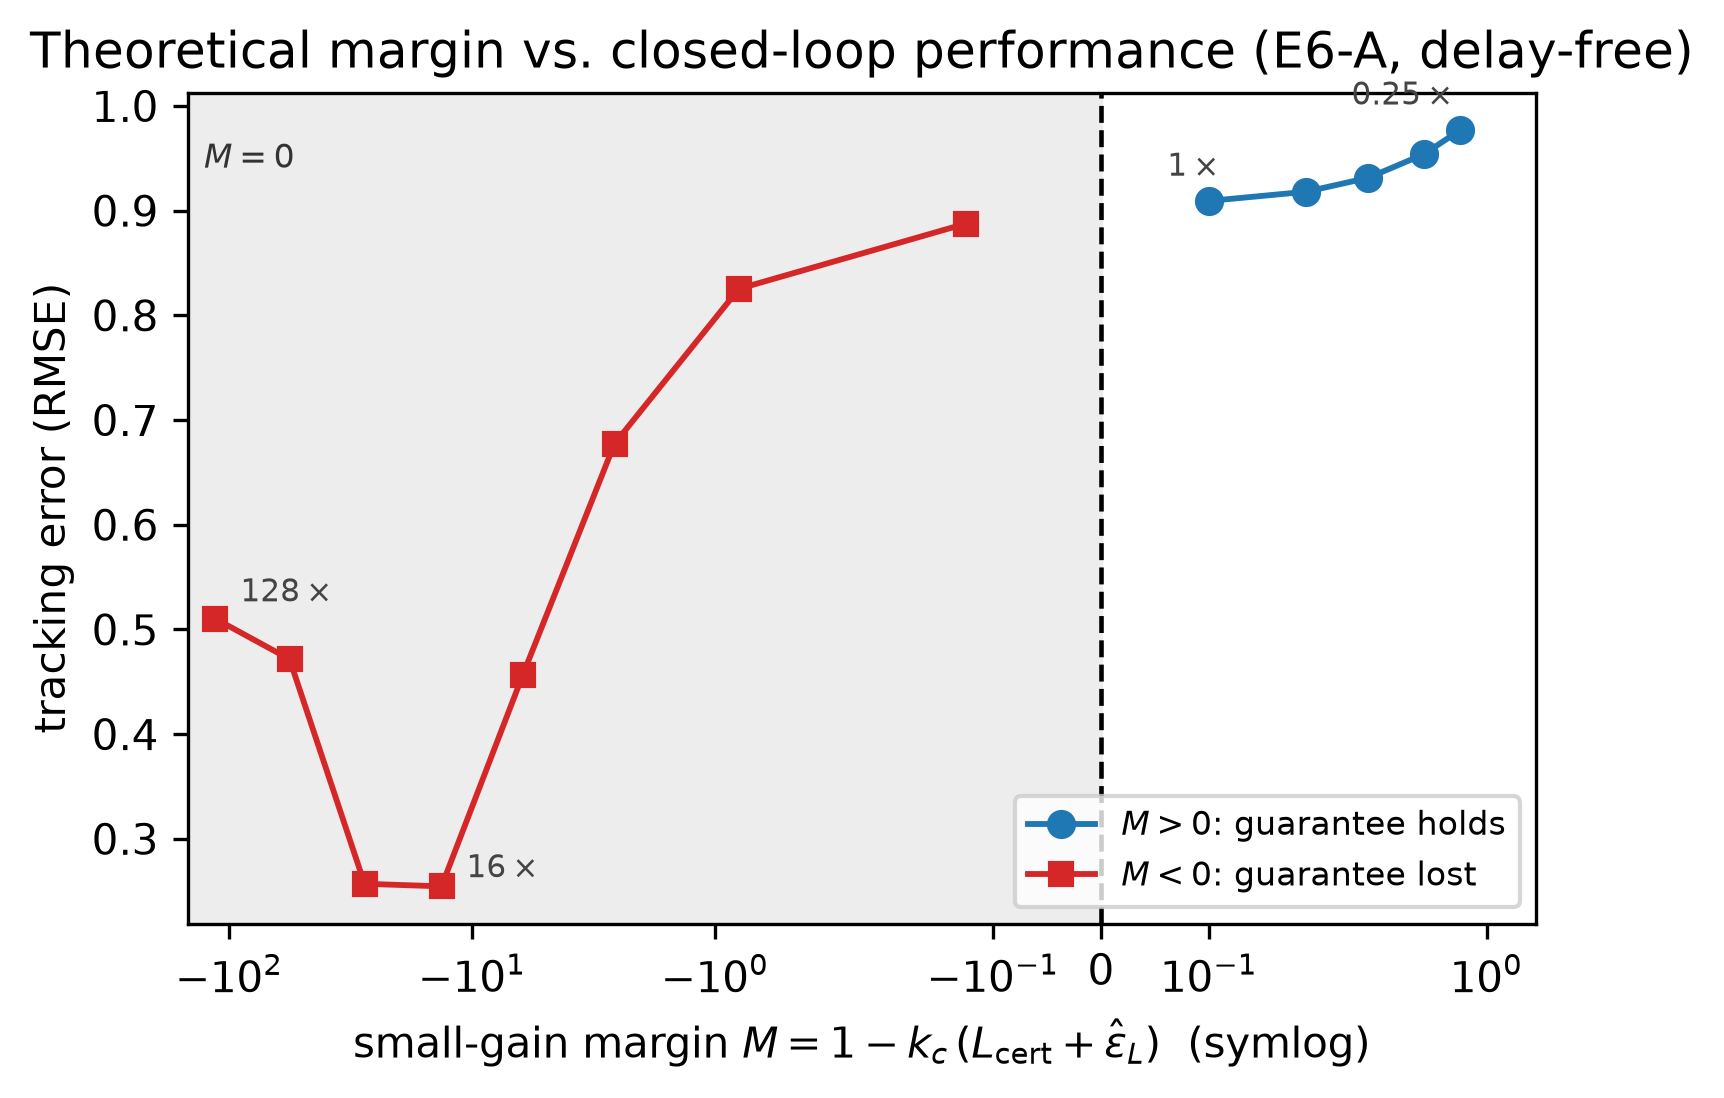
\includegraphics[width=0.72\textwidth]{fig12_margin_rmse.png}
\caption{Predicted margin versus closed-loop performance (E6-A,
one-step lag): each point is one controller gain of the sweep, plotted
against its predicted small-gain margin $M=1-k_c(\Lhat+\hat\epsL)$
(symmetric-log axis; annotated multiples of $k_c^{\mathrm{safe}}$). In
the shaded $M<0$ region the small-gain sufficient condition no longer
holds and the tracking error turns non-monotone; no divergence occurs at
any gain --- the margin predicts the loss of the guarantee, not the loss
of stability.}
\label{fig:marginrmse}
\end{figure}

\subsection{E7: Certificate--accuracy trade-off}
The certificate can be tuned explicitly through a target constraint, which
makes $\Lhat$ a \emph{designable} quantity rather than an emergent property of
training. A single-seed sweep over
$\lambda_{\mathrm{lip}}\in\{0.01,0.1,1,10\}$ at $\Ltarget=5$ leaves every
metric identical to machine precision (ID RMSE $0.0144$, $\Lhat=3.68$). A probe across ten independent runs (the default configuration and
the $+$Lip ablation of E5, five seeds each) explains why: the surrogate
$\tilde L$ stays within $[1.5,3.8]$ at every epoch, so the hinge penalty
$\max(0,\tilde L-\Ltarget)^2$ is
\emph{identically zero} and its gradient
never enters the loss. The invariance is therefore structural: at
$\Ltarget=5$ the penalty is a safeguard rather than a tuned regularizer.
This also explains the E5
ablation: the $+$Lip vs.\ bare difference reflects seed-level variability,
reproduced by an independent seed batch (ID RMSE $0.0128\pm0.0023$),
not a penalty that never activates.

The meaningful knob is $\Ltarget$. Sweeping it over $\{1.5,2,2.5,3,4,5\}$
with five seeds each (Table~\ref{tab:e7}, Fig.~\ref{fig:tradeoff}) traces the
trade-off: the certificate tracks the target down to $\Ltarget=1.5$
($\Lhat=1.53\pm0.08$, a $62\%$ compression from $4.00\pm0.24$) while the
in-distribution error stays essentially flat ($0.0116\pm0.0010$ vs.\
$0.0121\pm0.0015$) and the OOD error rises by about $20\%$
($0.0153\pm0.0015$ vs.\ $0.0127\pm0.0011$). The target is binding only at
the low end: for $\Ltarget\ge3$ the five-seed mean certificate
($2.46$, $3.58$, $4.00$) lies below its own target, so those rows
characterize largely unconstrained training, and only $\Ltarget\le2.5$
exerts downward pressure. The one point at which identification error
degrades is $\Ltarget=2.5$ (mean $0.0168\pm0.0065$); its certificate spread
($0.36$) is not the widest, which belongs to $\Ltarget=4$ ($0.77$), so the
two diagnostics do not coincide.

E10 verifies the pipeline at such a target: the LC side re-run at
$\Ltarget=2$ (five seeds) reaches $\Lhat=1.97\pm0.14$ with unchanged
identification ($0.0123\pm0.0015$); the calibrated design
$k_c=0.419$ still covers the sampled plant gain
($0.520$), the margin sweep reproduces the same
sign--degradation correlation, and conservatism drops to
$4.1\times$. Transfer at the same target retains its mean accuracy
(Duffing ID $0.0118\pm0.0008$, OOD $0.0149\pm0.0008$; pendulum ID
$0.0167\pm0.0082$, OOD $0.0260\pm0.0038$), at the price of a wider seed
spread than at the default target, one pendulum seed being an outlier.

\begin{table}[t]
\centering\small
\caption{Accuracy--certificate trade-off over the constraint target
$\Ltarget$ (mean $\pm$ std over 5 seeds each).}
\label{tab:e7}
\begin{tabular}{lccc}
\toprule
$\Ltarget$ & ID RMSE & OOD RMSE & $\Lhat$ \\
\midrule
1.5 & 0.0116$\pm$0.0010 & 0.0153$\pm$0.0015 & 1.53$\pm$0.08 \\
2.0 & 0.0123$\pm$0.0015 & 0.0152$\pm$0.0015 & 1.97$\pm$0.14 \\
2.5 & 0.0168$\pm$0.0065 & 0.0191$\pm$0.0063 & 2.10$\pm$0.36 \\
3.0 & 0.0117$\pm$0.0009 & 0.0141$\pm$0.0013 & 2.46$\pm$0.38 \\
4.0 & 0.0130$\pm$0.0022 & 0.0139$\pm$0.0028 & 3.58$\pm$0.77 \\
5.0 & 0.0121$\pm$0.0015 & 0.0127$\pm$0.0011 & 4.00$\pm$0.24 \\
\bottomrule
\end{tabular}
\end{table}

\begin{figure}[t]
\centering
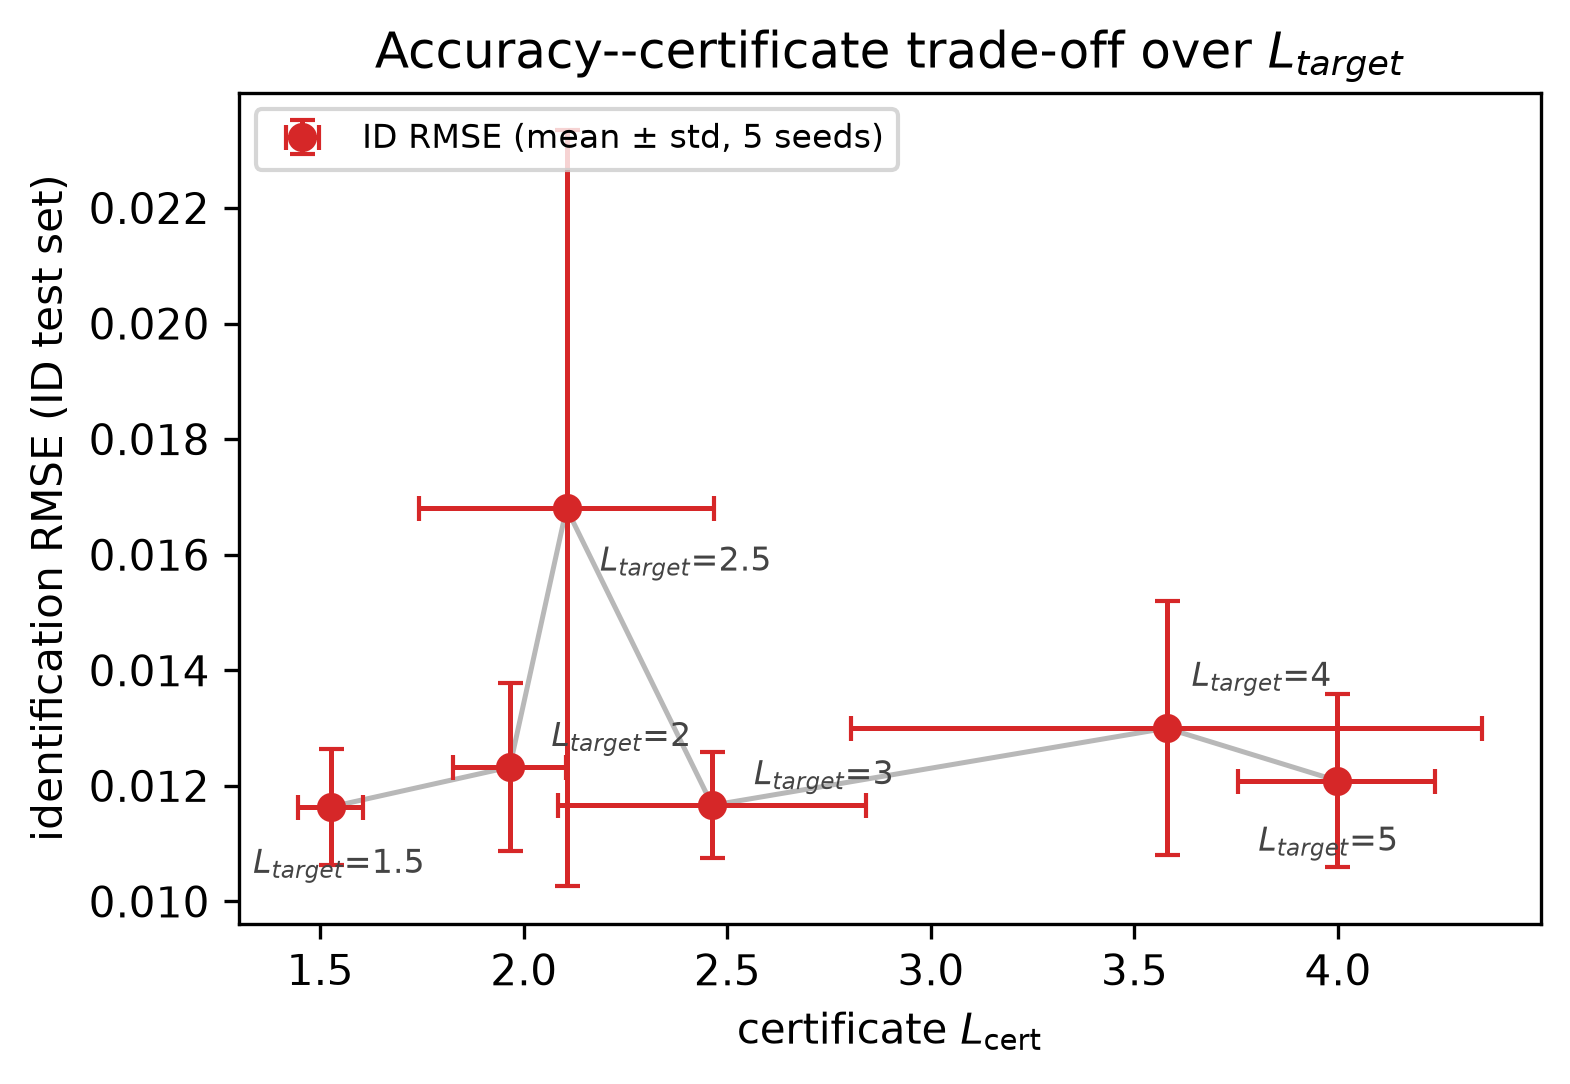
\includegraphics[width=0.62\textwidth]{fig10_tradeoff.png}
\caption{Accuracy--certificate trade-off (E7): identification RMSE
versus the resulting certificate $\Lhat$ as $\Ltarget$ sweeps
$\{1.5\text{--}5\}$ (mean $\pm$ std over 5 seeds; the curve is
parametrized by $\Ltarget$). Tightening the certificate by $62\%$ costs
essentially no in-distribution accuracy; the $\Ltarget=2.5$ point is the only
one at which identification error degrades.}
\label{fig:tradeoff}
\end{figure}

\subsection{E8: Transfer to Duffing and pendulum}
To show the pipeline is not tied to the MSD equation, E8 repeats the full
protocol on the Duffing oscillator $q''+\delta q'+\alpha_d q+\beta_d q^3=u$
and the nonlinear pendulum $\theta''+b\theta'+(g/l)\sin\theta=u$ (a
non-polynomial nonlinearity), with data, splits, architecture, and protocol
identical to E1; the OOD test extrapolates each
parameter range by $25\%$ ($\beta_d\in[4,5]$, $g/l\in[10,12.5]$;
Table~\ref{tab:e8}). Three observations: (i) LC-DeepONet attains the best
Duffing accuracy ($0.0110\pm0.0009$ vs.\ $0.0131\pm0.0024$) and matches the
unconstrained model on the pendulum ($0.0133\pm0.0008$), so the constraint
costs nothing here; (ii) the certificate emerges for both systems
($\Lhat=4.12\pm0.35$ and $3.37\pm0.08$) with no architecture change, a
quantity none of the baselines can emit; (iii) the FNO again shows the largest
Duffing errors, while all models are statistically tied on the pendulum OOD set,
where extrapolating the gravitational parameter dominates model
differences.

\begin{table}[t]
\centering\small
\caption{Transfer systems (E8; mean $\pm$ std over 5 seeds). OOD
extrapolates the parameter range by $25\%$. $\Lhat$ is reported only
for the model that produces it by construction.}
\label{tab:e8}
\begin{tabular}{llccc}
\toprule
System & Model & ID RMSE & OOD RMSE & $\Lhat$ \\
\midrule
Duffing   & FNO        & 0.0324$\pm$0.0008 & 0.0452$\pm$0.0025 & -- \\
          & DeepONet   & 0.0131$\pm$0.0024 & 0.0153$\pm$0.0031 & -- \\
          & \textbf{LC-DeepONet} & \textbf{0.0110$\pm$0.0009} & \textbf{0.0132$\pm$0.0010} & 4.12$\pm$0.35 \\
\midrule
Pendulum  & FNO        & 0.0184$\pm$0.0003 & 0.0246$\pm$0.0006 & -- \\
          & DeepONet   & 0.0133$\pm$0.0007 & \textbf{0.0242$\pm$0.0005} & -- \\
          & LC-DeepONet & \textbf{0.0133$\pm$0.0008} & 0.0248$\pm$0.0009 & 3.37$\pm$0.08 \\
\bottomrule
\end{tabular}
\end{table}

\subsection{E9: Long-horizon rollout}
Addressing the concern that short-horizon accuracy does not guarantee
long-horizon consistency, E9 evaluates each trained model on trajectories of
$T_{\mathrm{test}}\in\{4,6\}$\,s generated by the same protocol (same
parameter distribution and input class; Fig.~\ref{fig:longhorizon}). The full-horizon RMSE grows moderately for the
DeepONet family ($0.114\pm0.013\to0.147\pm0.011$ from $4$\,s to $6$\,s), and
the constrained model is statistically indistinguishable from the
unconstrained one at both horizons, so the certificate costs nothing in
long-horizon behaviour. The FNO baseline has larger errors at every time index
($0.153\pm0.021$, $0.185\pm0.030$), consistent with its larger measured
operator sensitivity in E3: a larger gain amplifies the accumulated mismatch
over longer horizons, exactly the behaviour a gain certificate exposes a
priori.

\begin{figure}[t]
\centering
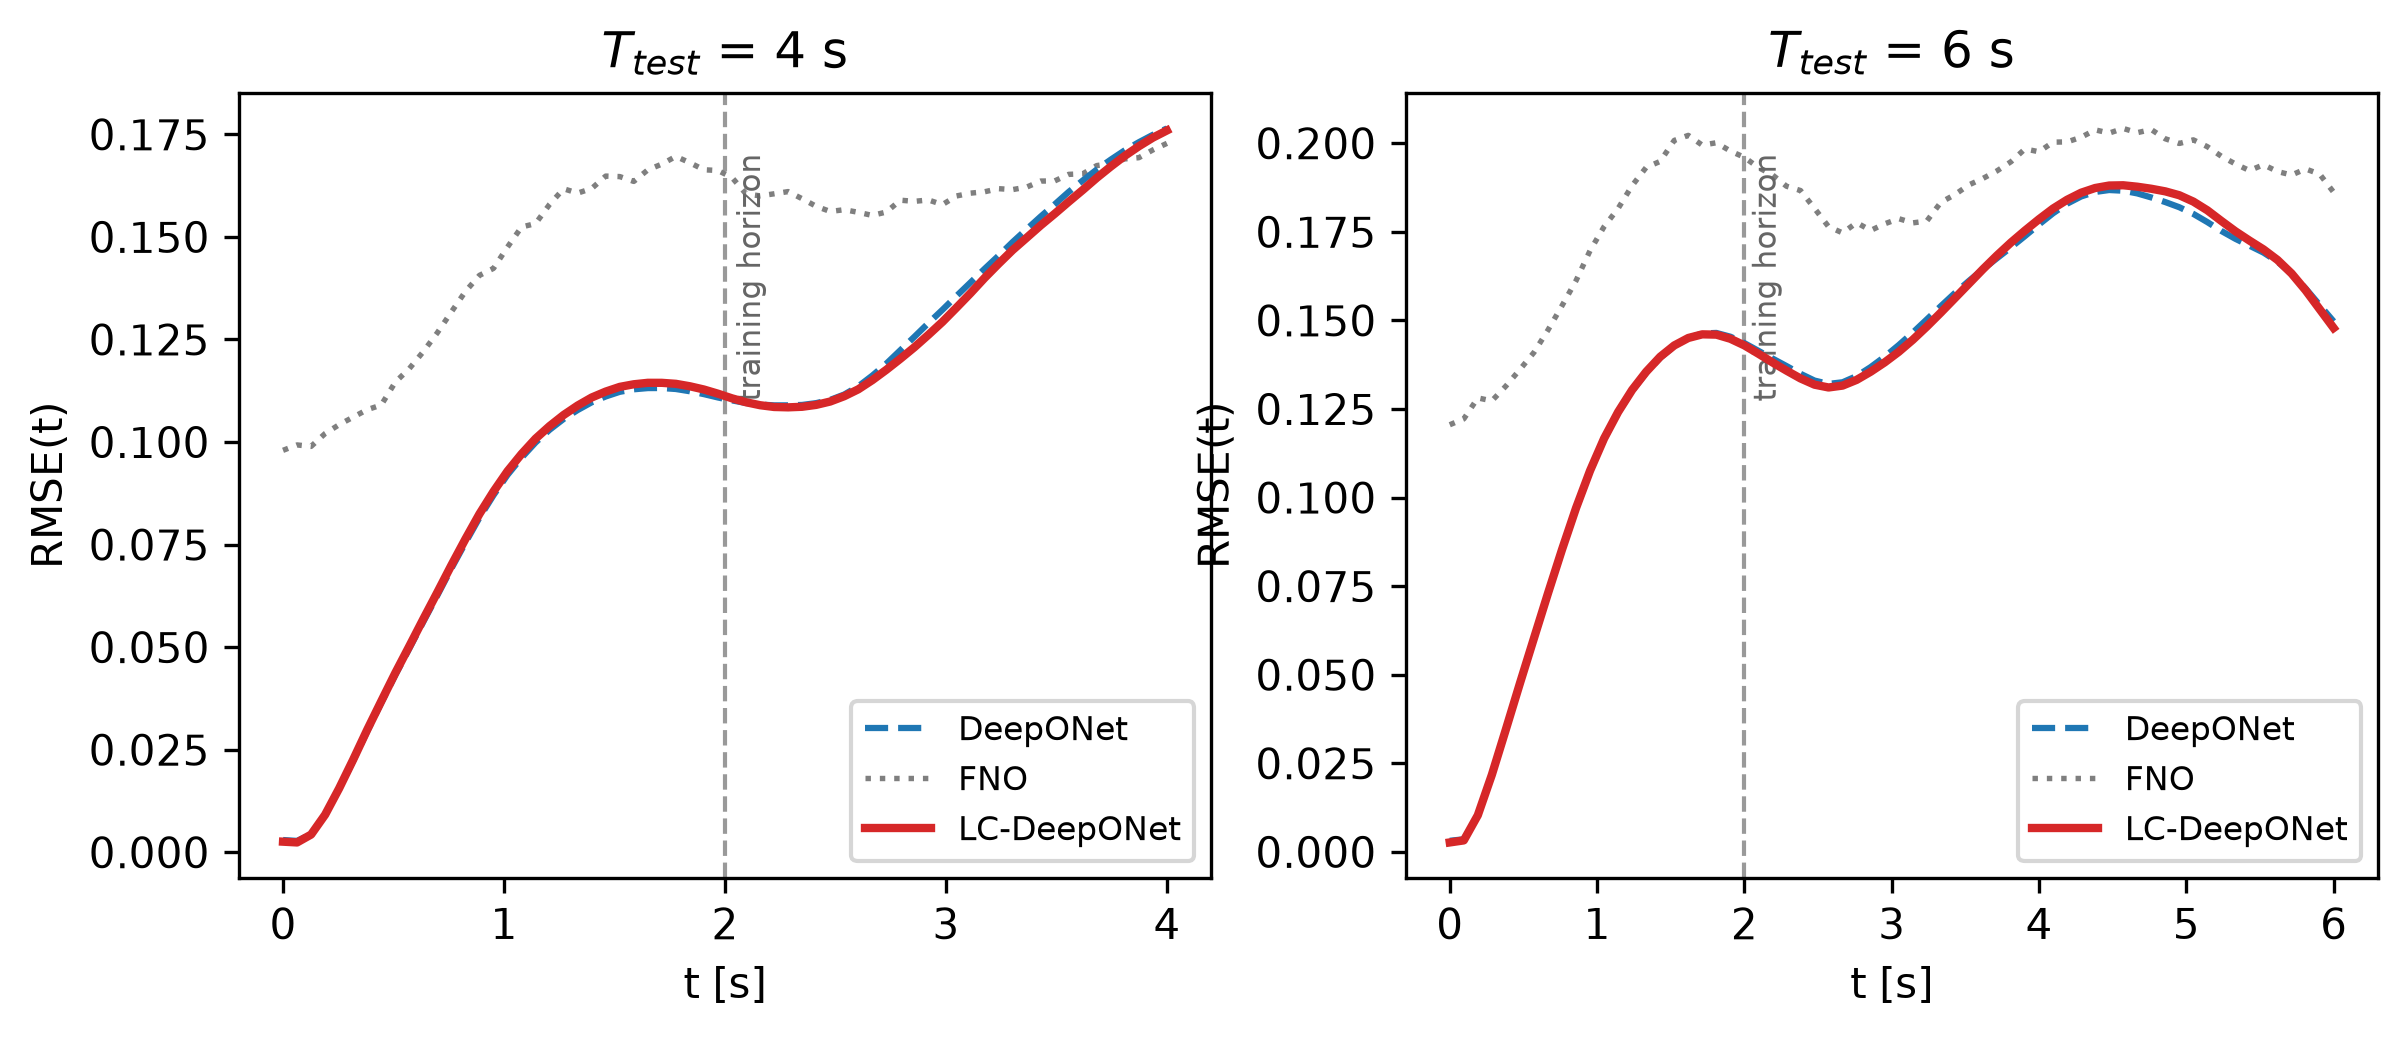
\includegraphics[width=\textwidth]{fig11_longhorizon.png}
\caption{Long-horizon rollout (E9): RMSE$(t)$ on test trajectories of
$T_{\mathrm{test}}=4$\,s (left) and $6$\,s (right); models trained on
$T=2$\,s windows (dashed line). The Lipschitz-constrained model tracks
its unconstrained counterpart at every time index, while the FNO
baseline is separated across the whole post-training-horizon region.}
\label{fig:longhorizon}
\end{figure}

% ---------------------------------------------------------------------
\section{Discussion}\label{sec:discussion}

\textbf{Conservatism.} Each ratio below divides an upper bound by a sampled \emph{lower} bound on the
plant gain and therefore overstates the true conservatism. The calibrated bound exceeds
the sampled plant-gain estimate by about $7\times$: for the single-run design
of E6-A, $3.73$ against $0.52$ at the box centre, and for the five-seed mean
of E6-C, $3.96$ against $0.517$ ($6.9\times$ at the worst corner, $4.03$
against $0.587$). A five-seed decomposition of the certificate batch
($\Lhat$ averaging $3.91$) localizes the source: the
branch layer product $\prod_i\sigma(W_i)$ averages $4.12$ and dominates,
while the trunk constant contributes $C_{\mathrm{T}}\approx0.96$ in the
Frobenius form, their product being $3.96$ against a batch-average bound of
$3.91$. Replacing the
Frobenius by the spectral norm --- the tight constant of the
aggregation step in Theorem~\ref{thm:cert} --- cuts the certificate by a
measured $15\%$ ($\Lhat=3.91\pm0.32\to3.31\pm0.29$ over five seeds),
bringing the factor to about $6$; the remaining gap is attributable to the
layer-product bound and the uniform-in-$u$ trunk constant.

\textbf{What the certificate buys, and what it costs.} The margin-blessed
design is deliberately conservative: the calibrated gain gives a tracking
error of $0.909$ at a one-step lag (E6-A) and $0.927$ with a $100$\,ms delay
(E6-C), whereas the uncertified high-gain design reaches $0.255$ at
$16\times$--$32\times$ and degrades to $2.97$ with an overshoot of $7.9$ once
delay is present (E6-B). The certificate therefore buys no tracking
performance on this plant. What it buys is a \emph{prior} screening rule (the
admissible gain and the region where the calibrated condition fails are known
before the loop is closed, from the weights plus one offline pass over plant
data), an interpretable margin whose predicted loss is observable in the
response, and a rule that transfers across systems (E8) and is insensitive to
its hyperparameters (E7).
The price is explicit: the ratios above are upper estimates, and
calibrating at the corner rather than the centre costs a further $2\%$
(E6-C); at a binding target the ratio falls to $4.1\times$ (E10). The certificate is therefore best read
as an offline risk-screening instrument: where plant iteration is expensive or
unsafe the conservative margin is the product, whereas where the smallest
tracking error is the goal the uncertified design wins.

\textbf{Assumption 1.} The residual-Lipschitz assumption is the linchpin
connecting identification error to stability. It concerns \emph{nature}
(plant--model mismatch), not the network, and can be discharged in two ways:
\emph{a priori}, on a small-signal envelope, via
Proposition~\ref{prop:apriori} for the MSD class (data-free but
amplitude-restricted, Remark~\ref{rem:price}); or \emph{a posteriori}, at the
operating amplitude, via the estimate of Remark~\ref{rem:epsL} --- a lower
bound, so the resulting designs are empirically calibrated rather than
certified, and the variant $\gamma_s\hat\epsL$ tightens them at a
proportional gain cost.

\textbf{Generalization.} Under the 512-sample, 5-seed OOD protocol the
Lipschitz constraint shows no measurable generalization penalty; this is an
empirical observation, not a guarantee.

\textbf{Limitations.} Simulation-only study; single-output systems; the design
rule is replicated over five networks (E6-D) but each corner loop of E6-C still
uses one design gain ($\Lhat$ ranges over $3.68$--$4.33$); the nominal
sweeps are anchored at the box centre, and
the box is covered analytically only by the conservative a priori route; the
loop delay exposes the margin--performance correlation but is not analyzed
within the small-gain framework (delay is infinite-dimensional and outside
the stated assumptions); and the closed-loop statements are empirically
calibrated rather than formally certified, since no validated upper bound on
$\mathrm{Lip}(E)$ at the operating amplitude is available.

% ---------------------------------------------------------------------
\section{Conclusion}\label{sec:conclusion}
We turned the small-gain theorem's hypothesis into a trainable object.
LC-DeepONet learns a nonlinear input--output operator while emitting a
computable $\Ltwo$ gain certificate; an explicit residual-Lipschitz
assumption converts identification error into a plant gain bound; and the
bound yields a small-gain feedback condition --- certified in the model
gain, empirically calibrated in the residual term --- whose practical value is
demonstrated by gain-margin sweeps on a parameter-uncertain nonlinear plant,
including a re-calibration at all eight corners of the uncertainty box, where
the design gain shifts by only $2\%$ and every closed loop remains stable;
the same training and certification pipeline is applied to Duffing
and pendulum systems without system-specific architecture changes, is
insensitive to its hyperparameters, and costs nothing in
long-horizon rollout. Only the model-gain statement is formally certified;
the plant- and loop-level statements are design rules validated in
simulation. Future work
includes tightening the certificate (local or adaptively weighted bounds),
a priori bounds on $\epsL$ for structured plant classes, transfer to hardware
testbeds, and extension to infinite-dimensional (PDE) plants where the
operator certificate is the natural currency.

% ---------------------------------------------------------------------
\section*{Statements and Declarations}

\subsection*{Ethical considerations}
Not applicable. This is a purely numerical study on simulated dynamical
systems, with no human participants, human data, or animals; no ethics
approval was required.

\subsection*{Consent to participate}
Not applicable.

\subsection*{Consent for publication}
Not applicable.

\subsection*{Declaration of conflicting interests}
The author declared no potential conflicts of interest with respect to the
research, authorship, and/or publication of this article.

\subsection*{Funding}
No financial support was received for the research, authorship, or
publication of this article.

\subsection*{ORCID iD}
Peng Chen \url{https://orcid.org/0009-0004-9021-6039}

\subsection*{Data availability}
All datasets analysed in this study are generated deterministically by the
released code (fixed random seeds; no external data are used). The aggregated
CSV results reported in all tables and figures are included in the repository,
and the complete raw results are regenerated by the experiment scripts.

\section*{Code availability}
The complete implementation---models, training pipeline, certificate
computation, closed-loop simulation, and all experiment scripts covering
E1--E10 together with the M3 certificate audit---is available at
\url{https://github.com/chenpeng0326/LC-DeepONet}; a versioned DOI
snapshot will be deposited in a public archive on acceptance. Every quantitative claim is
regenerable from the released scripts and committed result files
(\texttt{results/*.csv}); \texttt{README.md} maps each table and figure to
its generating script and result file, and
\texttt{results/e6\_design\_provenance.csv},
\texttt{results/e6s\_design\_per\_seed.csv} and
\texttt{results/e10\_lt2\_design\_provenance.csv} record every scalar behind
the closed-loop designs (per seed for E6-D), so that the E6 and E10 numbers
can be recomputed without retraining.



% ---------------------------------------------------------------------
\begin{thebibliography}{99}

% Sage Vancouver (numbered) style: entries appear in the order of first citation
% in the text; in-text citations are superscript numbers (sagev class option).
\bibitem{lu2021deeponet}
L.~Lu, P.~Jin, G.~E. Karniadakis,
``DeepONet: Learning nonlinear operators for identifying differential
equations based on the universal approximation theorem of operators,''
\emph{Nature Machine Intelligence}, vol.~3, pp. 218--229, 2021.

\bibitem{li2021fno}
Z.~Li, N.~Kovachki, K.~Azizzadenesheli, et~al.,
``Fourier neural operator for parametric partial differential equations,''
in \emph{International Conference on Learning Representations (ICLR)}, 2021.

\bibitem{lanthaler2022error}
S.~Lanthaler, S.~Mishra, G.~E. Karniadakis,
``Error estimates for DeepONets: a deep learning framework in infinite
dimensions,''
\emph{Transactions of Mathematics and Its Applications}, vol.~6, no.~1,
Art.\ no.\ tnac001, 2022. DOI: 10.1093/imatrm/tnac001.

\bibitem{moya2025conformal}
C.~Moya, A.~Mollaali, Z.~Zhang, L.~Lu, G.~Lin,
``Conformalized-DeepONet: a distribution-free framework for uncertainty
quantification in deep operator networks,''
\emph{Physica D: Nonlinear Phenomena}, vol.~471, Art.\ no.\ 134418, 2025.
DOI: 10.1016/j.physd.2024.134418.

\bibitem{bhan2024bypassing}
L.~Bhan, Y.~Shi, M.~Krstic,
``Neural operators for bypassing gain and control computations in PDE
backstepping,''
\emph{IEEE Transactions on Automatic Control}, vol.~69, no.~8,
pp. 5310--5325, 2024.

\bibitem{krstic2024observer}
M.~Krstic, L.~Bhan, Y.~Shi,
``Neural operators of backstepping controller and observer gain functions
for reaction--diffusion PDEs,''
\emph{Automatica}, vol.~164, Art.\ no.\ 111649, 2024.

\bibitem{xiao2024output}
Y.~Xiao, Y.~Yuan, B.~Luo, X.~Xu,
``Neural operators for robust output regulation of hyperbolic PDEs,''
\emph{Neural Networks}, vol.~179, Art.\ no.\ 106620, 2024.
DOI: 10.1016/j.neunet.2024.106620.

\bibitem{lv2025cascaded}
K.~Lv, J.~Wang, Y.~Cao,
``Neural operator approximations for boundary stabilization of cascaded
parabolic PDEs,''
\emph{International Journal of Adaptive Control and Signal Processing},
vol.~39, no.~7, pp. 1503--1520, 2025. DOI: 10.1002/acs.3902.

\bibitem{qi2024pide}
J.~Qi, J.~Zhang, M.~Krstic,
``Neural operators for PDE backstepping control of first-order hyperbolic
PIDE with recycle and delay,''
\emph{Systems \& Control Letters}, vol.~185, Art.\ no.\ 105714, 2024.
DOI: 10.1016/j.sysconle.2024.105714.

\bibitem{miyato2018spectral}
T.~Miyato, T.~Kataoka, M.~Koyama, Y.~Yoshida,
``Spectral normalization for generative adversarial networks,''
in \emph{Advances in Neural Information Processing Systems (NeurIPS)}, 2018.

\bibitem{pauli2021lipschitz}
P.~Pauli, A.~Koch, J.~Berberich, P.~Kohler, F.~Allg{\"o}wer,
``Training robust neural networks using Lipschitz bounds,''
\emph{IEEE Control Systems Letters}, vol.~6, pp. 121--126, 2022.
DOI: 10.1109/LCSYS.2021.3050444.

\bibitem{brunton2016sindy}
S.~L. Brunton, J.~L. Proctor, J.~N. Kutz,
``Discovering governing equations from data by sparse identification of
nonlinear dynamical systems,''
\emph{Proceedings of the National Academy of Sciences}, vol.~113, no.~15,
pp. 3932--3937, 2016.

\bibitem{raissi2019pinn}
M.~Raissi, P.~Perdikaris, G.~E. Karniadakis,
``Physics-informed neural networks: A deep learning framework for solving
forward and inverse problems involving nonlinear partial differential
equations,''
\emph{Journal of Computational Physics}, vol.~378, pp. 686--707, 2019.

\bibitem{lusch2018deep}
B.~Lusch, J.~N. Kutz, S.~L. Brunton,
``Deep learning for universal linear embeddings of nonlinear dynamics,''
\emph{Nature Communications}, vol.~9, Art.\ no.\ 4950, 2018.

\bibitem{masti2021learning}
V.~Masti, A.~Bemporad,
``Learning nonlinear state-space models using autoencoders,''
\emph{Automatica}, vol.~129, Art.\ no.\ 109666, 2021.

\bibitem{kolter2019learning}
J.~Z. Kolter, G.~Manek,
``Learning stable deep dynamics models,''
in \emph{Advances in Neural Information Processing Systems (NeurIPS)}, 2019.

\bibitem{chang2019neural}
Y.-C. Chang, N.~Roohi, S.~Gao,
``Neural Lyapunov control,''
in \emph{Advances in Neural Information Processing Systems (NeurIPS)}, 2019.

\bibitem{liang2024learning}
Y.~Liang, J.~Zhang, H.~Zhao, H.~Su, X.~Cui,
``A learning-based approach to event-triggered guaranteed cost control
for completely unknown nonlinear systems,''
\emph{Transactions of the Institute of Measurement and Control},
vol.~46, no.~6, pp. 1203--1218, 2024. DOI: 10.1177/01423312231185383.

\bibitem{zheng2024adaptive}
X.-Y.~Zheng,
``Adaptive neural control for non-strict feedback stochastic nonlinear
systems with input delay,''
\emph{Transactions of the Institute of Measurement and Control},
vol.~46, no.~1, pp. 104--115, 2024. DOI: 10.1177/01423312231169561.

\bibitem{hewing2020learning}
L.~Hewing, K.~P. Wabersich, M.~Menner, M.~N. Zeilinger,
``Learning-based model predictive control: Toward guaranteed safety and
performance,''
\emph{IEEE Control Systems Magazine}, vol.~40, no.~5, pp. 100--127, 2020.

\bibitem{desoer1975feedback}
C.~A. Desoer, M.~Vidyasagar,
\emph{Feedback Systems: Input--Output Properties}. Academic Press, 1975.

\bibitem{khalil2002nonlinear}
H.~K. Khalil, \emph{Nonlinear Systems}, 3rd~ed. Prentice Hall, 2002.

\end{thebibliography}


\end{document}
